% This is the Reed College LaTeX thesis template. Most of the work
% for the document class was done by Sam Noble (SN), as well as this
% template. Later comments etc. by Ben Salzberg (BTS). Additional
% restructuring and APA support by Jess Youngberg (JY).
% Your comments and suggestions are more than welcome; please email
% them to cus@reed.edu
%
% See http://web.reed.edu/cis/help/latex.html for help. There are a
% great bunch of help pages there, with notes on
% getting started, bibtex, etc. Go there and read it if you're not
% already familiar with LaTeX.
%
% Any line that starts with a percent symbol is a comment.
% They won't show up in the document, and are useful for notes
% to yourself and explaining commands.
% Commenting also removes a line from the document;
% very handy for troubleshooting problems. -BTS

% As far as I know, this follows the requirements laid out in
% the 2002-2003 Senior Handbook. Ask a librarian to check the
% document before binding. -SN

%%
%% Preamble
%%
% \documentclass{<something>} must begin each LaTeX document
\documentclass[12pt,twoside]{reedthesis}
% Packages are extensions to the basic LaTeX functions. Whatever you
% want to typeset, there is probably a package out there for it.
% Chemistry (chemtex), screenplays, you name it.
% Check out CTAN to see: http://www.ctan.org/
%%
\usepackage{graphicx,latexsym}
\usepackage{amsmath}
\usepackage{amssymb,amsthm}
\usepackage{longtable,booktabs,setspace}
\usepackage{chemarr} %% Useful for one reaction arrow, useless if you're not a chem major
\usepackage[hyphens]{url}
% Added by CII
\usepackage{hyperref}
\usepackage{lmodern}
\usepackage{float}
\floatplacement{figure}{H}
% End of CII addition
\usepackage{rotating}

% Next line commented out by CII
%%% \usepackage{natbib}
% Comment out the natbib line above and uncomment the following two lines to use the new
% biblatex-chicago style, for Chicago A. Also make some changes at the end where the
% bibliography is included.
%\usepackage{biblatex-chicago}
%\bibliography{thesis}


% Added by CII (Thanks, Hadley!)
% Use ref for internal links
\renewcommand{\hyperref}[2][???]{\autoref{#1}}
\def\chapterautorefname{Chapter}
\def\sectionautorefname{Section}
\def\subsectionautorefname{Subsection}
% End of CII addition

% Added by CII
\usepackage{caption}
\captionsetup{width=5in}
% End of CII addition

% \usepackage{times} % other fonts are available like times, bookman, charter, palatino


% To pass between YAML and LaTeX the dollar signs are added by CII
\title{A Big Data Analysis of Pokémon Battling}
\author{Samuel D. Olson}
% The month and year that you submit your FINAL draft TO THE LIBRARY (May or December)
\date{May 2017}
\division{Mathematics and Economics}
\advisor{Prof.~Andrew Bray}
%If you have two advisors for some reason, you can use the following
% Uncommented out by CII
\altadvisor{Prof.~Yan Lau}
% End of CII addition

%%% Remember to use the correct department!
\department{Mathematics and Economics}
% if you're writing a thesis in an interdisciplinary major,
% uncomment the line below and change the text as appropriate.
% check the Senior Handbook if unsure.
\thedivisionof{The Established Interdisciplinary Committee for}
% if you want the approval page to say "Approved for the Committee",
% uncomment the next line
\approvedforthe{Committee}

% Added by CII
%%% Copied from knitr
%% maxwidth is the original width if it's less than linewidth
%% otherwise use linewidth (to make sure the graphics do not exceed the margin)
\makeatletter
\def\maxwidth{ %
  \ifdim\Gin@nat@width>\linewidth
    \linewidth
  \else
    \Gin@nat@width
  \fi
}
\makeatother

\renewcommand{\contentsname}{Table of Contents}
% End of CII addition

\setlength{\parskip}{0pt}

% Added by CII
  %\setlength{\parskip}{\baselineskip}
  \usepackage[parfill]{parskip}

\providecommand{\tightlist}{%
  \setlength{\itemsep}{0pt}\setlength{\parskip}{0pt}}

\Acknowledgements{
I wanted to thank everyone working for Pokémon Showdown for the
opportunity to work with a rich dataset that continues to pose
challenges well beyond the realm of Pokémon battling.
}

\Dedication{
This work is dedicated to all past, current and future members of The
Rocking Chair.
}

\Preface{

}

\Abstract{
\par  

This study attempts to answer a question pertaining to game strategies:
is it beneficial to pursue strategies that do not immediately damage an
opponent? Furthermore: is the impact of these strategies dependent upon
when the moves are used? These questions are tested using data from a
popular online Pokémon battling game, Pokémon Showdown. This study tests
whether the use of specific moves positively contribute to a player's
likelihood of winning a battle. This study finds surprisingly uniform
results. Evidence shows that when players utilize moves that do not
directly damage their opponent, they have a higher likelihood of winning
a game. Additionally, moves considered complementary to these strategies
positively impact a player's likelihood of winning a game more than only
utilizing moves that do not directly damage their opponent. Furthermore,
this study provides evidence that these effects are more pronounced when
a player pursues these strategies earlier in a game, defined as within
the first five turns of a game.
}

	\usepackage{setspace}
	\doublespacing
% End of CII addition
%%
%% End Preamble
%%
%

\begin{document}

% Everything below added by CII
      \maketitle
  
  \frontmatter % this stuff will be roman-numbered
  \pagestyle{empty} % this removes page numbers from the frontmatter

      \begin{acknowledgements}
      I wanted to thank everyone working for Pokémon Showdown for the
      opportunity to work with a rich dataset that continues to pose
      challenges well beyond the realm of Pokémon battling.
    \end{acknowledgements}
  
  
      \hypersetup{linkcolor=black}
    \setcounter{tocdepth}{2}
    \tableofcontents
  
      \listoftables
  
      \listoffigures
  
      \begin{abstract}
      \par  
      
      This study attempts to answer a question pertaining to game strategies:
      is it beneficial to pursue strategies that do not immediately damage an
      opponent? Furthermore: is the impact of these strategies dependent upon
      when the moves are used? These questions are tested using data from a
      popular online Pokémon battling game, Pokémon Showdown. This study tests
      whether the use of specific moves positively contribute to a player's
      likelihood of winning a battle. This study finds surprisingly uniform
      results. Evidence shows that when players utilize moves that do not
      directly damage their opponent, they have a higher likelihood of winning
      a game. Additionally, moves considered complementary to these strategies
      positively impact a player's likelihood of winning a game more than only
      utilizing moves that do not directly damage their opponent. Furthermore,
      this study provides evidence that these effects are more pronounced when
      a player pursues these strategies earlier in a game, defined as within
      the first five turns of a game.
    \end{abstract}
  
      \begin{dedication}
      This work is dedicated to all past, current and future members of The
      Rocking Chair.
    \end{dedication}
  
  \mainmatter % here the regular arabic numbering starts
  \pagestyle{fancyplain} % turns page numbering back on

  \chapter{Pokémon Showdown and The Pokémon
  World}\label{pokemon-showdown-and-the-pokemon-world}
  
  \section{Introduction}\label{introduction}
  
  The world of Pokémon began in 1996 with the pair of games Pokémon Red
  and Green. For Western audiences, the latter game would become known as
  Pokémon Blue. These two games introduced a unique system turn-based game
  that continues to define the franchise of Pokémon games. Numerous other
  games have attempted to copy the Pokémon battling format, but none have
  been able to equal its widespread appeal and dedicated player base. With
  each successive iteration, new items, Pokémon types, and of course new
  species of Pokémon are added to the Pokémon lexicon. As a result, the
  world of Pokémon has continued to grow and evolve into one of the
  largest video games franchises to date. The most recent iteration of
  Pokémon games, Pokémon Sun and Moon, have continued Pokémon's commercial
  and historical trend of turning profits while adding layers to an
  already complex system of battling.
  
  Since 2011 the program Pokémon Showdown has offered a simplified version
  of Pokémon games. This simplified version allows players to exclusively
  battle one another, replicating the most recent iteration of the Pokémon
  games in the process. This has allowed players to hone and test their
  Pokémon battling skills through the years. With well-over 10,000 daily
  registered users and counting, this program has become the go-to program
  to test and practice Pokémon battling strategies in the ultimate pursuit
  of becoming the very best that no one ever was.
  
  However, before any formal analysis of Pokémon battling is discussed,
  the battling system of Pokémon must be rigorously detailed for laymen
  and theorists alike.
  
  First and foremost, each Pokémon battle occurs exclusively between two
  players. Each of the two players has a team composed of six Pokémon. For
  the purposes of analysis, teams with duplicate Pokémon will not be
  considered, namely because such teams are not allowed in ranked battles
  (and not included in the data considered in this study). As such, teams
  are composed of six distinct Pokémon. As a point of note, only battles
  in the `Anything Goes' category allow any Pokémon to be used, including
  duplicate species within a player's team. Furthermore, depending on the
  battle format the team of six Pokémon is either randomly assigned or
  dictated by the player. The format being considered in this study,
  Overused (abbreviated OU), provides an example format where players
  dictate their team composition. A number of different battle formats
  exist beyond OU and Anything Goes, including Random Battles (abbreviated
  Randbats), giving a cumulative total of 59 different battle formats at
  the time this study was conducted.
  
  \begin{figure}[htbp]
  \centering
  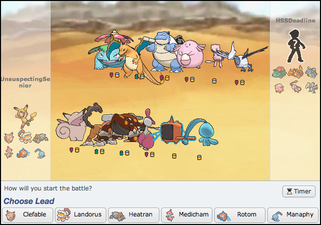
\includegraphics{pic1.png}
  \caption{The Beginning of a Battle}
  \end{figure}
  
  Regardless of the battle format, each turn each player simultaneously
  makes a decision for the Pokémon they have on the field. The decisions
  are then executed. The order of play is decided by a comparison of the
  moves each player selects. Priority is given first to priority moves and
  then, if neither player selected a priority move for the turn, by a
  comparative assessment of the speeds of the two Pokémon. If each player
  uses a move with the same priority, then the comparative assessment of
  speed is used to determine who attacks first.
  
  The potential moves Pokémon are able to execute have a wide variety of
  effects (the finer details are discussed in Chapter 2). Regardless of
  the damage or effects of the executed moves, once a player's Pokémon
  loses all of its health, an event referred to as fainting, the player
  must switch into another Pokémon. If a player has no other Pokémon to
  switch into, the battle ends. As would be expected, the player whose
  Pokémon have all fainted loses the battle. Conversely, the player who
  eliminates all of their opponent's Pokémon wins.
  
  Furthermore, each Pokémon has at most four possible moves to chose from
  during any turn of a battle. Whenever a player has at least two Pokémon
  that have not fainted, they have additional choice to switch into
  another Pokémon. Doing so counts as the player's action for the turn. As
  a result, players almost always have five different choices to make each
  turn.
  
  There are still a number of other details that are relevant to consider
  beyond those already mentioned. Namely, while some information is fixed
  during the battle, including the opposing players team composition, some
  variables of interest are case-specific. These include what moves an
  opposing Pokémon has already used, and consequently revealed, along with
  a given Pokémon's held item, its ability, and a slew of other variables.
  However, similar to the different type of moves a Pokémon can choose
  from, these points will be detailed in the Chapter 2.
  
  That being said, to formally analyze Pokémon battling the game itself
  must be formally denoted in game theoretic terms. This will aid in both
  describing the game and in highlighting its complexity. With this in
  mind, it bears noting that there are only two outcomes to any battle:
  One player wins and the other loses. Because of this, Pokémon battling
  is by definition a zero-sum game. However, it is important to note that
  there some distinctions between how a player can win or lose a game.
  Though the game ends when all of the Pokémon on one team have fainted,
  any player has the choice to forfeit the game any time before this
  occurs. Thus, the two ways to win or lose a battle are either by
  forfeiture or by having all of their Pokémon faint; this latter outcome
  is referred to as a full game. Additionally, there is the potential for
  a game to result in a draw. However, draws result in a neutral payoff as
  neither player raises or lowers their ranking after a draw. By contrast,
  when a player wins a battle their rank increases, while conversely if
  they lose their rank decreases.
  
  \section{Game Theory of Pokémon}\label{game-theory-of-pokemon}
  
  Within the scope of game theoretic terms, it is vital to note that each
  player is able to see all past decisions made over the course of a
  battle. Additionally, battles only last a finite number of turns.
  Speaking to the former point, players are able to recall not only their
  past decisions but also those of their opponent, including how much
  damage was done by a specific move during a given turn. In the format
  analyzed in this study, players even know the composition of their
  opponent's team from the very beginning of the match, as shown in Figure
  1.1. More generally however, this information is available at any time
  during the battle, making Pokémon battling a perfect recall game.
  Furthermore, as each game is composed of a sequence of turns, Pokémon
  battling is a sequential game.
  
  \begin{figure}[htbp]
  \centering
  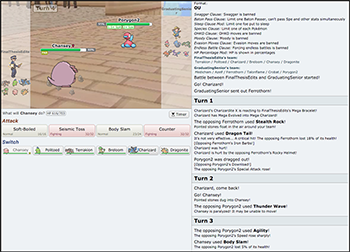
\includegraphics{pic5c.png}
  \caption{Information Available After Two Turns}
  \end{figure}
  
  The points pertaining to the availability information allude to a unique
  trait of Pokémon battling that further details the type of game Pokémon
  battling is: An incomplete information game. Though the extent of
  incompleteness is format specific, each player is given limited
  information about the opposing player's team at the beginning of the
  battle. After each turn, players learn not only the different moves each
  opposing Pokémon has, but also their abilities, held items, and
  sometimes what other Pokémon compose the opposing team (if the format is
  Randbats). Generally speaking, there is almost always new information
  revealed each turn.
  
  Taken together, Pokémon battling is a special case of a sequential,
  zero-sum two-player game with incomplete information and perfect recall.
  As Pokémon battling lends itself to a discussion of imperfect
  information, it is all the more vital to consider the role of decision
  making within the context of sequential games. However, it is vital to
  note that this study will not do so using expansive game trees or
  comparison of payoff tables. Namely this is done due to computational
  limitations, which were ever present throughout the research process.
  
  However, the extent to which player strategies are revealed from
  information is an open topic of discussion, both in the post-estimation
  analysis if this study and current game theory literature. Naturally,
  the analysis of such a topic relies upon at least one a priori
  assumption, namely that player strategies are revealed by their past
  decisions. However, whether player strategies are rational and
  consistent is another matter entirely, and one that is not explicitly
  addressed. Nonetheless, it is important to note that incorporating such
  information into players own decision-making complicates analysis and is
  a central topic in analyzing player strategies specific to Pokémon
  battling.
  
  Game theoretic considerations aside, there are also important
  computational notes to detail. In this regard, initial computations and
  analysis focused on the distribution of turn lengths, i.e.~the length of
  games played when one player forfeited or had all of their Pokémon faint
  and the corresponding distribution of game lengths. These initial
  computations revealed that there were a number of battles that lasted
  less than one turn, which were then pruned from later models and
  analysis. Following this, moves are categorized by their type,
  specifically whether a specific move is a ``setup'' move or may be
  considered complementary to a ``setup'' move. These two types of moves
  are considered in greater detail in Chapter 2. Following this, I gauge
  the effectiveness of using specific moves on the empirical probability
  that using such move corresponded to a winning outcome.
  
  Overall I explore the decision-making process involved in Pokémon
  battling, specifically moves that are considered patient and moves
  considered complementary to patient moves. By incorporating tenants of
  behavioral economics and game theory, I hope to highlight not only the
  empirical probabilities of winning associated with specific move sets,
  but also analyze how and why such events may contribute to a higher
  lilkihood of winning a battle. More specifically, I will continue the
  recent trend of `Big Data' analysis to explore macro trends in player's
  decision making processes. In doing so I hope to answer two main
  questions: Does utilizing patient strategies positively influence the
  likelihood of winning a Pokémon battle, and are these findings
  generalizable across specifications? In the context of Pokémon battling,
  is a player is better off by deciding to use one type of entry hazard
  over another and are these findings generalizable across when in the
  battle the moves were used?
  
  \section{Literature Review}\label{literature-review}
  
  Scant rigorous or academic research has been conducted within the scope
  of Pokémon-related topics. The most frequent publications have typically
  focused on Pokémon as a cultural phenomena or have been official
  strategy guides for the various Pokémon games published by Nintendo
  affiliates. Importantly, these strategy guides do not detail Pokémon
  battling strategies, although they do detail the numerous Pokémon
  species, items, and moves available in each game. Thus, strategy guides
  provide a foundational background about the Pokémon, moves, and other
  basic information but do not provide clear formulations of general
  battling strategies. Some recently publications have come close though.
  
  Academic papers that have focused Pokémon battling have developed and
  analyzed algorithms to simulate Pokémon battling and play against human
  players in the program Pokémon Showdown. The first paper of this kind
  gives a rudimentary background on Pokémon battling and focuses
  explicitly on 1v1 battle simulations (Gildardo 2013). However, in a
  detailed analysis of one particular one-on-one scenario the author is
  single minded and only focuses on one-on-one Pokémon battles.
  Furthermore, Gildardo (2013) does not consider other potential variants
  on Pokémon abilities or item pairings. In this regard, Gildardo's
  article does not go into great detail on the many variants of Pokémon
  battling, as highlighted by the exclusion of teams of Pokémon.
  
  This point notwithstanding, since Gildardo (2013) there has been one
  other notable publication that focuses on Pokémon battling. This
  publication focuses on the creation and analysis of algorithms within
  the context of Pokémon battling; the article additionally goes into
  greater detail on battling strategies while incorporating comparative
  analysis of the different algorithms used to play against human
  opponents (Ho et al. 2016). Though Ho et al. 2016 focused on what is
  currently a previous iteration of Pokémon Showdown, the iteration of
  Pokémon Showdown is fundamentally the same as that of the data used in
  this study. Nonetheless, the paper does have some shortcomings as well.
  Namely, the algorithms used would never select a move whose type would
  be not very effective against the opponent's fielded Pokémon. This point
  will be detailed later, but needless to say such a decision is not
  always the preferred one, especially if the moves being used are entry
  hazards.
  
  Furthermore, on the subject of different versions of Pokémon Showdown,
  relevant documentation of the past iterations of Pokémon Showdown are
  available at the program's website. The website for Pokémon Showdown
  provides a hub for information ranging from Pokémon battling basics to
  specific battle format descriptions. Similar to all information
  mentioned thus far, replays and ladder ranking are available publically.
  Furthermore, the site provides Pokémon usage statistics and a damage
  calculator for aspiring Pokémon battlers.
  
  As noted previously, game theory vernacular has not entered into
  discussions on Pokémon battling strategies, at least in any formal
  setting. Applying such concepts to the context of Pokémon battling
  offers a formal foundation to discuss strategies and test hypotheses. In
  this regard, there are three main areas of game theory that intersect in
  the analysis of Pokémon battling. These three areas of interest include
  the interpretation of Pokémon battling as a zero sum game, the role of
  incomplete information, and the implications of Pokémon battling as a
  non-cooperative game. These three topics actively influence the
  decision-making process associated with Pokémon battling.
  
  A central factor involved in the decision making process as it relates
  to game theory is the role of information, specifically how players
  incorporate information revealed each turn into their strategies. As
  information is revealed each turn, including the four moves an opposing
  Pokémon has, each Pokémon's ability, held item, and a number of other
  factors, it is vital for players to determine if the information they
  just received in a given turn is relevant. Simply put, players need to
  decide if the information they just received provides any insight into
  their opponent's strategy. Overall, this speaks to Pokémon being a game
  with imperfect information. As such, it is not possible to apply
  Zermelo's theorem, though its negation provides insight as to the
  possible existence of a weakly dominating strategy (Schwalbe et al.
  2001). The method to empirically test such strategies is by tracking the
  use of specific moves, in this study entry hazards and complementary
  moves, and testing whether players that used specified move sets won
  more games than players that did not utilize such move sets.
  
  This being said, concepts from game theory are not the only relevant
  ideas for analyzing Pokémon battling. In the context of exploring the
  frequency of players switching Pokémon will necessarily invoke concepts
  from behavioral economics as well as game theory. Relevant to the field
  of behavioral economics, the concept of ``keeping doors open'' is an
  interesting concept to explore in regards to Pokémon battling. The
  concept of ``keeping doors'' open is explored in Chapter 6 of Ariely's
  work Predictably Irrational, giving an idea of what the expected results
  may be in the context of Pokémon battling. Specifically, as players may
  decide to preemptively switch Pokémon in the hopes of having that
  Pokémon later in the battle, they may arrive at suboptimal outcomes. Via
  application of Ariely's empirical results, players may prefer to keep
  certain Pokémon available until the end of the battle, even if doing so
  incurs costs and/or reduces their chances of winning. Though this
  concept is not explicitly tested, this study tackles a similar though
  contrapositive point by empirically testing whether moves that do not
  necessarily incur damage the turn they are used result in a higher
  likelihood of winning a battle. By doing so, this study tests whether
  players are better off when they only use damaging moves, or
  specifically non-entry hazard moves. However, before tackling how to
  formulate a testable hypothesis, some of the finer details of Pokémon
  battling must be highlighted.
  
  \chapter{Game Description}\label{game-description}
  
  The data used is a compilation of battle logs taken from the Pokémon
  Showdown servers. The data spans the entirety of December 25th, 2015 to
  December 27th of the same year. No battle logs are incomplete, i.e.~none
  of the daily data entries are empty, though some are excluded for their
  turn length. Each battle effectively serves as two observations in the
  dataset, one observation for each player. Overall, there were no
  dramatic overhauls done to the OU format or the overall Pokémon battling
  system used in this study. However, some adjustments have been made
  since the time covered in this study and will be highlighted in the
  analysis portion of the study.
  
  Furthermore, only ranked games are included in the dataset. Ranked
  battles are battles that count towards a players global ranking in
  Pokémon Showdown. For each battle, players stand to gain or lose ranking
  points depending on whether they win or lose the battle.
  
  As noted in the Literature Review, a number of different Pokémon
  databases redirect users to the host site of Pokémon Showdown. The name
  is this site is Smogon University. The website for Smogon University
  offers a wide variety of resources, similar to those found at the
  Pokémon Showdown website. Most importantly the Smogon forums are a
  prominent site for discussion of Pokémon battling strategies, along with
  detailing what Pokémon compose specific battle formats.
  
  \section{Pokémon Battling Basics}\label{pokemon-battling-basics}
  
  The Pokémon battle starts with one Pokémon being sent out from each
  player's team. For the purposes of the data used in this study, one
  Pokémon is sent out from each opponent. This totals two Pokémon being
  active at any given point in the battle. Following this, each Pokémon
  has 4 moves to choose from, along with the option to switch to a
  different Pokémon (when applicable). After both players make a decision,
  the moves are weighted for priority and speed to determine the order of
  play. If both players decide not to switch, one Pokémon will attack the
  other, after which the next Pokémon will do the same if it has not
  fainted. After each move has been executed the turn ends and the process
  is repeated. When one of the Pokémon faints, the player whose Pokémon
  fainted will be prompted to select another Pokémon from the bench. The
  first player to lose all of their Pokémon loses the battle.
  
  However, before the nitty gritty details are explained it is important
  to make a concession. The entirety of the Pokémon battling system, even
  that used in the data, is not included in this analysis. The number of
  cases that deviate from the rules detailed below are either not included
  in the competitive format, or are generally inconsequential to the
  scenarios and strategies considered in this study.
  
  \subsection{Battle Formats}\label{battle-formats}
  
  The data used for this study includes only one battling format: OU. The
  two most frequently used formats are OU and Randbats respectively, at
  least as indicated from preliminary fact-finding. Both formats have
  teams of six Pokémon and only allow one Pokémon to be out at any given
  time. While both battle formats are subsets of what are known as single
  battles, only OU will be highlighted in greater detail.
  
  The OU format includes team composition. By including team composition,
  players are able to decide what Pokémon to include on their team, the
  moves of each Pokémon, and other parameters such as held items and
  abilities. However, there are still some restrictions placed on players.
  Specific species of Pokémon are barred from use, notably Pokémon
  classified as ``Ubers''. Uber Pokémon include a large number of
  legendary Pokémon, along with some mega-Pokémon. Additionally, certain
  ``hidden'' abilities are restricted, limiting the possible Pokémon
  abilities a specific species may use for a given format.
  
  \subsubsection{Format-Specific Pokémon}\label{format-specific-pokemon}
  
  There are a number of other battle formats that are not analyzed in the
  current study. Nonetheless, a brief overview of these is germane in
  relation to the different Pokémon explicitly studied. The order of
  `tiers' is as follows: Uber, OU, BL, UU, NU, and Limbo, where BL stands
  for Borderline, UU stands for Under Used, and NU stands for Never Used.
  A number of species in tiers below OU are used in the battles observed
  in the dataset. Just as Ubers allows use of Pokémon that are from OU
  battles, so too do the other tiers of Pokémon battling, i.e.~UU allows
  use of NU Pokémon. However, there are a number of Pokémon that `belong'
  to a given tier, insomuch as they are considered staple Pokémon of that
  format. To reduce the list of 600+ Pokémon, the roster of Pokémon
  considered in this study are the 415 Pokémon that are considered staple
  Pokémon for the tiers spanning OU to Limbo. This effectively reduces the
  number of Pokémon that are considered competitive, along with doing so
  in a manner that is systematic to the players of the games considered.
  That being said, it's important to delve into some Pokémon-specific
  topics that are general to the battling system, not necessarily related
  to specific battle formats.
  
  \subsection{Pokémon Types}\label{pokemon-types}
  
  Typeage is a unique characteristic to Pokémon battling. Currently there
  are 18 distinct types. These include normal, fire, water, electric,
  grass, ice, fighting, poison, ground, flying, psychic, bug, rock, ghost,
  dragon, dark, steel, and fairy. Both moves and Pokémon are given a type
  attribute, though moves are only one type. Additionally, while a move
  may only be one of the 18 types, a Pokémon can be at most two different
  types at once.
  
  However, some of these combinations are not found in Pokémon. From the
  initially possible 171 Pokémon type combinations, 18 choose 2 plus 18
  monotypes, there are actually only 133 types that a player may encounter
  or chose from (as 38 type combinations had not yet been used during
  2015). It is also worth noting that some Pokémon are able to change type
  during a battle, but for the purposes of analysis these Pokémon will be
  considered special cases and will be briefly touched upon in Chapters 3
  and 4.
  
  The typeage of each Pokémon influence not only the potential weaknesses
  of each Pokémon, but also the amount of damage that type-specific does.
  Each Pokémon has at least one and at most two types. If a Pokémon uses a
  damaging move whose type corresponds to the typeage of the Pokémon that
  used it, that Pokémon gets a same type attack bonus, abbreviated as a
  ``stab'' bonus. This causes the move to do 50\% more damage, potentially
  100\% if the Pokémon also has the ability Adaptability.
  
  \subsection{Pokémon Attributes}\label{pokemon-attributes}
  
  Generally, there are a number of factors that are specific to each
  Pokémon. Some of these factors are considered static, meaning that they
  do not and cannot change over the course of the battle. These types of
  factors are defined as ``Fixed'' attributes. However, some factors such
  as the base statistics of a Pokémon are fixed at the beginning of the
  battle and \emph{can} change over the course of a battle. There are also
  a number of factors that are able to generally change over the course of
  a battle. Such factors, by constrast, are defined as ``Variable''
  attributes. The terminology is largely taken from Ho et al. (2016) for
  ease of appropriability. The attributes are detailed in the order given.
  
  \subsection{Pokémon Fixed Attributes}\label{pokemon-fixed-attributes}
  
  Fixed attributes include the typeage of a Pokémon, the four moves each
  Pokémon specie has, the item the Pokémon holds, the Pokémon's ability,
  the level of the Pokémon, and the Pokémon's base statistics. However,
  there are exceptions to the rules for each of these attributes except
  for the level of the Pokémon. Every fixed attribute and its respective
  exception(s) will be considered in the order listed.
  
  First and foremost is the typeage of a Pokémon, detailed previously. One
  scenario where a Pokémon can change its type is specific to a Pokémon's
  ability. Both Protean and Color Change are abilities that are able to
  change a friendly Pokémon's typeage. The former ability changes the
  Pokémon Kecleon's type to that of the move that affected (or hit) it,
  whereas the latter ability turns its type into the typeage of the move
  that just was just used by the Pokémon Greninja. These two abilities are
  specific to Kecleon and Greninja. Furthermore, there are moves that able
  to make the opponents Pokémon into a water, grass, or ghost Pokémon (on
  top of their previous typeage) if they use the moves Soak, Forest's
  Curse, and Treat-Or-Treat respectively.
  
  Each Pokémon's set moves are also fixed during a battle. The exception
  to this occurs when a Pokémon runs out of power points, denoted as PP,
  for all of its four moves. Every move has a set limit to the number of
  times it can be used, though the number of times a move can be used
  varies across the set of moves. At this point the Pokémon is only able
  to use the move struggle. The move is a physical attack that will also
  the damage the user of the move. The struggle is real.
  
  Pokémon are able to hold one item at the beginning of the match. Pokémon
  may also lose their held item either by being hit by the move Knock-off,
  which knocks the opponent's Pokémon's item off, or by using their held
  item. Some held items are able to be consumed for a one-time effect.
  This scenario includes the consumption of berries, which offer a variety
  of different effects to the Pokémon holding it. For example, if a
  Pokémon is given a status condition, a condition detailed in the
  following section, from an opposing Pokémon while holding a Lum berry,
  the berry will be consumed and the Pokémon's status condition will be
  cured. The player does not actually control when the berry will be
  consumed, as the consumption of the berry is dependent upon what moves
  an opponent uses on said Pokémon. This example highlights an important
  characteristic of some held-items: some items may only be used once and
  are discarded after their initial use.
  
  One of the most important items that a Pokémon can hold is an item that
  allows the Pokémon to mega-evolve. When a Pokémon mega-evolves, it
  increases its base statistics, changing its ability, and even changing
  the typeage of the Pokémon. This special case of item holding is a focus
  of this study. Additionally, only one mega-Pokémon is allowed on a team
  at once, making variables that account for the different mega-Pokémon
  independent by nature. An example of a Pokémon that has undergone
  mega-evolution is shown in Figure 2.1.
  
  \begin{figure}[htbp]
  \centering
  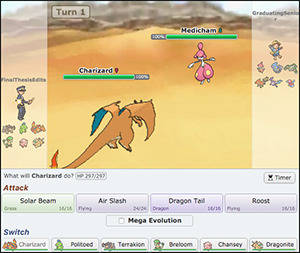
\includegraphics{pic4c.png}
  \caption{First Turn Options}
  \end{figure}
  
  Similar to items, a Pokémon can only have one ability at a time.
  However, by contrast to a Pokémon's held item a Pokémon always has an
  ability. A Pokémon cannot have no ability. Nonetheless, Pokémon may have
  their ability swapped with another Pokémon's. This scenario only occurs
  a Pokémon makes physical contact with Yamask or Cofagrigus, at which
  point its ability is swapped with Mummy. Mummy will only change a
  physically-attacking Pokémon's ability; it has no other effect.
  
  The level of a Pokémon varies between one and one-hundred. The higher
  the level, the better the base statistics for a given Pokémon,
  specifically in comparison to lower levels of that given Pokémon. Base
  statistics are divided into six categories. These categories include
  (baseline) health, attack, special attack, defense, special defense, and
  speed. There is further nuance with the inclusion of Pokémon natures and
  Individual Values, or IVs. These factors influence the base statistics
  of each Pokémon. However due to the sheer number of trivial combinations
  of IV spreads and nature choices, these two factors will not be a
  pivotal aspect to the framework and analysis of Pokémon battling.
  Nonetheless, the volatility of these baseline stats will be considered
  as a variable attribute.
  
  \subsection{Pokémon Variable
  Attributes}\label{pokemon-variable-attributes}
  
  Variable Attributes include boosts or reductions to a Pokémon's base
  statistics, the status condition of the Pokémon, the volatile status of
  the Pokémon, the current health of the Pokémon, and whether the Pokémon
  is currently active.
  
  The former-most attribute directly influences how effective an active
  Pokémon is able to be in battle. Pokémon are able to learn and use moves
  that can boost their own status or ones that reduce their opponents.
  However, these moves are only able to influence a Pokémon's attack,
  special attack, defense, special defense, or speed. For example, the
  move Swords Dance raises its users attack status so long as the Pokémon
  remains active. The move may be used multiple times, but is only
  effective until it boosts or lowers its target's baseline stat by 3 or
  1/3 respectively.
  
  Status conditions are composed of a variety of statuses. Pokémon that
  suffer a status condition are either burned, frozen, paralyzed,
  poisoned, badly poisoned, or have fallen asleep. A Pokémon can only
  suffer from one status condition at a time, although a Pokémon can
  suffer from multiple status conditions during a battle if it overcomes
  the first status condition.
  
  Each of these statuses is distinct, though there are similarities
  between being poisoned or badly poisoned. A Pokémon that is just
  poisoned will take damage equal to 1/8th of its maximum HP at the end of
  each turn. By comparison a Pokémon that is badly poisoned takes n/16th
  of its maximum HP at the end of the nth turn the Pokémon has been badly
  poisoned. A Pokémon that is poison-type or steel-type is unable to be
  poisoned, and if a Pokémon has the ability Poison Heal it is healed
  1/8th of its maximum HP at the end of each turn.
  
  If a Pokémon is burned it takes 1/8th of its maximum HP in damage at the
  end of the turn. This has recently been changed to 1/16th of its maximum
  HP per turn, but this is just a passing point of note. Regardless of the
  amount of damage done to the burned Pokémon, the burned Pokémon's
  physical attacks do half damage. The exception to this rule is if the
  affected Pokémon has the ability Guts. Additionally, a fire-type Pokémon
  cannot be burned.
  
  In a similar vein to being burned, a paralyzed Pokémon has its speed
  reduced to 1/4th of its base speed. Furthermore, a Pokémon that is
  paralyzed has a 1/4 chance of not being able to move during its move.
  This event is referred to as being ``fully paralyzed''. Furthermore,
  electric-type Pokémon are unable to be paralyzed, and if a Pokémon has
  the ability Lightning Rod it's special attack is boosted by 1.5 its base
  level. Additionally, ground-type Pokémon cannot be paralyzed, just as
  they are not affected by electric-type moves.
  
  A Pokémon that has fallen asleep is unable to use its moves except for
  the moves Snore and Sleep Talk. A Pokémon falls asleep for one to five
  turns. However, if a Pokémon purposely puts itself to sleep using the
  move rest, it is asleep for exactly two turns. If a Pokémon has either
  of the abilities Vital Spirit or Insomnia, it cannot be put to sleep.
  
  Lastly, there is the status condition of being frozen. Similar to
  previous typed statuses, ice type Pokémon are immune to becoming frozen,
  as are Pokémon with the ability Magma Armor. There is no set number of
  turns that a Pokémon can be frozen, but if a frozen Pokémon is hit by
  fire-type moves or the move scald is thaws out and is no longer frozen.
  
  Volatile statuses are similar to status conditions, except that the
  volatile status will be negated by switching out the affected Pokémon.
  Similar to status conditions, a Pokémon can only be affected by one
  volatile status at a time. Another important point to consider is that a
  Pokémon can suffer from both a volatile status \emph{and} a status
  condition, i.e.~a Pokémon can be both paralyzed and confused. That being
  said, the most common form of volatile status is confusion. A Pokémon is
  confused for one to four turns, during which time the confused Pokémon
  has a 50\% chance to hurt itself instead of executing its move for the
  turn. A Pokémon may also be encored, meaning that it has to use the same
  move it just moved for 3 turns.
  
  Only currently active Pokémon are able to execute moves. Likewise, only
  active Pokémon may be damaged. Beyond this there is not anything else to
  detail in regards to the current health and activity of a Pokémon that
  is exclusive to variable attributes.
  
  \subsection{\texorpdfstring{Environmental Variables (``Patient
  Moves'')}{Environmental Variables (Patient Moves)}}\label{environmental-variables-patient-moves}
  
  There is one more class category to detail that is relevant to the
  analysis of Pokémon battling. This category is the role of the
  environment in battling and is a central focus of this study's analysis
  of Pokémon battling. Though related to the different types of moves and
  abilities a Pokémon has, including both fixed and variable attributes,
  the environment is not specific to any one move, ability, or specie of
  Pokémon and as such must be highlighted separately from the previous
  attributions.
  
  The most prominent environmental variables to consider are what are
  referred to as ``set-up'' moves. These moves include Stealth Rock,
  Spikes, Toxic Spikes, Sticky Web, Light Screen, and Reflect. The latter
  two are different from the rest of the set-up moves in that they only
  last five turns, eight if the user was holding Light Clay when the move
  was used. When these moves are employed, the active Pokémon's special
  defense and defense are raised by one stage -or is increased by 1.5-
  respectively between Light Screen and Reflect. However, Light Screen and
  Reflect are not considered in the model specifications because they have
  a limited effect.
  
  The former four set-up moves are a focal point of analysis and are in a
  category of moves known as entry hazard moves. Entry hazards are
  considered patient moves in this study due to their indirect effects,
  namely that they do not directly damage opposing Pokémon the turn they
  are used. These moves are of particular note because they can last for
  the entirety of a given battle. Once these moves are used, only certain
  moves or switches are able to eliminate them. Generally, using the move
  rapid spin or defog will eliminate the entry hazards, along with causing
  other effects. However, if a Pokémon uses defog, both their and their
  opponent's entry hazards will be eliminated. By contrast, rapid spin
  only eliminates entry hazards affecting the users team.
  
  However, both defog and rapid spin are not included in the analysis.
  Instead, moves that are seen as supplemental to entry hazards are
  considered. The four moves that are considered supplemental to entry
  hazards include Dragon Tail, Circle Throw, Whirlwind, and Roar. The
  latter two moves only switch out the opposing player's Pokémon, whereas
  the former two moves will damage the opponent's active Pokémon and then
  switch them out. All of these moves force the opponent's active Pokémon
  to switch into another random Pokémon on their team. This process
  necessarily requires the opponent to have another Pokémon to switch
  into. However, as players always know how many more Pokémon are
  available for both their and their opponent's teams, an underlying
  assumption is that these moves are not used trivially, i.e.~when the
  opposing player only has one Pokémon left on their team.
  
  Moreover, there is still the matter of detailing entry hazards. To begin
  with, both Stealth Rock and Sticky Web can only be used once during a
  battle, at least until previous uses of either are eliminated by use of
  moves such as Rapid Spin. However, each of these entry hazards have
  different effects. Specific to the latter, Pokémon that enter the field
  after Sticky Web is employed have their speed lowered by one stage, or
  2/3rd their baseline level. This only applied to grounded, or
  non-flying, Pokémon however. By contrast, Stealth Rock will damage any
  Pokémon that enters the field after it is used. The amount of damage
  done to the Pokémon depends on the type effectiveness of rock-type
  moves, as Stealth Rock is a rock-type move. In ascending order, Stealth
  Rock will do 3.125\%, 6.25\%, 12.5\%, 25\%, and 50\% of the affected
  Pokémon's maximum health according to type effectiveness. This
  corresponds to 0.25x, 0.5x, 1x, 2x, and 4x damage respectively.
  
  Similar to Sticky Web, spikes only affect non-flying type Pokémon.
  However, spikes will inflict damage to Pokémon that switch in instead of
  afflicting them with a volatile status condition. The amount of damage
  is dependent upon the number of layers of spikes active on the field.
  Spikes may be applied a maximum of three times. One layer of spikes will
  damage the opposing Pokémon by 1/8th of its maximum HP, while two layers
  will deal 1/6th, and three layers will do 1/4th of the opposing
  Pokémon's maximum health.
  
  Lastly is toxic spikes that, just like spikes and sticky web, only
  affect grounded Pokémon with a status condition. However, toxic spikes
  are able to be applied two times. The first layer of toxic spikes will
  poison opposing Pokémon that switch in, while two layers of toxic spikes
  will badly poison Pokémon that switch in (that is, if the Pokémon that
  switches in is able to be poisoned). Just like most other entry hazards,
  toxic spikes only affects grounded Pokémon.
  
  \chapter{Empirical Results}\label{empirical-results}
  
  \section{Model Specification}\label{model-specification}
  
  As Pokémon battles included in the dataset have only two outcomes, we
  may estimate the probability of winning using a standard probit model.
  There are minor differences between using a logit and probit models, so
  the decision to use a probit model is simply a personal choice.
  Additionally, each battle effectively serves as two separate
  observations, or one observation for each player. As for the models, let
  Y denote the outcome of any battle for a given player, where Y takes the
  value of 0 if the player loses the battle and 1 if the player wins. To
  identify whether specific moves and Pokémon choices differentially
  impact the probability of winning a game, we define the dependent
  variable of the models used as \(f^{-1}(P(Y=1))\), where \(f^{-1}\) is
  the probit function.
  
  Surprisingly, there were no draws in the dataset, perhaps alluding to a
  small likelihood for a draw to occur. Nonetheless, to address the
  question of whether any entry hazards positively impact a player's
  likelihood of winning, we develop a number of different probit models.
  
  We begin with whether a specific move was used by a player in a battle.
  Let the set of all entry hazards be denoted \(S_1\) and let the set of
  all complementary moves be denoted \(S_2\). We define the full set of
  moves as \(S\) where \(S\) is defined as follows: S =\{Stealth Rock,
  Spikes, Toxic Spikes, Sticky Web, Dragon Tail, Roar, Circle Throw,
  Whirlwind\}.\\
  Furthermore, \(S_1\)=\{Stealth Rock, Spikes, Toxic Spikes, Sticky Web\}.
  By construction, \(S_2 = S/S_1\), as by definition \(S=S_1 \cup S_2\).
  This distinction is important for later model specifications.
  Additionally, for simplicity let the elements of the set \(S\), \(S_1\)
  and \(S_2\) be defined by the acronym of each move, i.e.~Stealth Rock is
  denoted SR.
  
  Then, define a count variable on the set S that takes the value of how
  many times a specified move is used in a battle. As an example, let
  \(M_{SR}\) be the variable that counts the number of times Stealth Rock
  was used in a battle. The variable takes value 1 when Stealth Rock is
  used once in a battle and 0 if it was not used at all by a player in a
  battle. We define the variables \(M_S\) , \(M_{TS}\) , \(M_{SW}\) ,
  \(M_{DT}\) , \(M_R\) , \(M_{CT}\) , and \(M_W\) similarly. These
  variables will be interacted with one another in later models, but they
  also provide strategic value singularly. For this reasons they will be
  included in the preliminary model, which is given by:
  
  \((1): f^{-1}(P(Y=1)) = \alpha + \sum_{i \in S} \beta_i(M_i)\)
  
  This study focuses particularly on the interactions and repeated use of
  the specified moves. Interactions in particular focus on Stealth Rock,
  because it directly damages Pokémon that switch in and because it can
  only be used once, making interaction terms easier to interpret than
  interactions with moves that can be used multiple times. Nonetheless,
  the squared term for Stealth Rock is included in the second model to
  test whether reapplying the move is an effective battling strategy. This
  includes cases were the battle environment is cleared. That being said,
  the model for including the squared term of moves is given as follows:
  
  \((2): f^{-1}(P(Y=1)) = \alpha + \sum_{i \in S} \beta_i(M_i) + \sum_{i \in S} \iota_i(M_i)^2\)
  
  We then include interactions between different moves and their squared
  terms. The corresponding model (3) is given by:
  
  \((3): f^{-1}(P(Y=1)) = \alpha + \sum_{i \in S} \beta_i(M_i) + \sum_{i \in S} \iota_i(M_i)^2 + \sum_{j \in S/{SR}} \theta_j(M_{SR} \times M_j) + \sum_{j \in S/{SR}} \lambda_j(M_{SR} \times (M_j)^2)\)
  
  These models have not yet included the vast variety of species composing
  teams. Before defining these models, we must first define the set of all
  competitive Pokémon and mega-Pokémon. To begin with the former, let the
  set of all competitive Pokémon be denoted \(P\), where
  \(P=\{Abomasnow,...,Zygarde\}\). The full list of Pokémon and their
  frequency of use in the dataset is included in the Appendix. There are
  415 elements in the set \(P\) and 39 in the set \(G\), where \(G\) is
  the set of all Mega-Pokémon allowed in the OU format. Let \(P_1\) be the
  first element in the set of Pokémon \(P\). Let the numerical index apply
  for all 415 Pokémon. Similarly define \(G_1\) as the first mega-Pokémon
  in the set \(G\). Then we index the set of 39 mega-Pokémon numerically.
  
  Following the indexing of the set of Pokémon and mega-Pokémon, we
  construct a number of variables that act as indicators for whether the
  Pokémon was used in a battle by a player. Hence, we define the variable
  for using the first Pokémon on the competitive roster as \(PU_1\), which
  takes the value 1 if the first Pokémon on the competitive roster is used
  and 0 otherwise. This is applied iteratively across all 415 competitive
  Pokémon. Furthermore, let \(GU_1\) denote the variable indicating if the
  first mega-Pokémon in the mega-Pokémon roster is used in a battle. This
  construction is applied to the set of 415 Pokémon and 39 mega-Pokémon.
  
  Before examining the interactions between a team's composition of
  Pokémon and specific moves, there needs to be a formal model that
  accounts for the impact of a Pokémon choice on the likelihood of winning
  a battle. Respective to the variables outlined previously, we have:
  
  \((4): f^{-1}(P(Y=1)) = \alpha + \sum_{i \in S} \beta_i(M_i) + \sum_{i \in S} \iota_i(M_i)^2 + \sum_{j \in S/{SR}} \theta_j(M_{SR} \times M_j) + \sum_{j \in S/{SR}} \lambda_j(M_{SR} \times (M_j)^2) + \sum_{l \in P} \gamma_l(PU_l)\)
  
  Thirty nine different Pokémon can turn into mega-Pokémon however. To
  test whether a Pokémon negatively or positively impacts the probability
  of winning, the next model specification includes mega-Pokémon within
  the roster of competitive Pokémon. The model is given by:
  
  \((5): f^{-1}(P(Y=1)) = \alpha + \sum_{i \in S} \beta_i(M_i) + \sum_{i \in S} \iota_i(M_i)^2 + \sum_{j \in S/{SR}} \theta_j(M_{SR} \times M_j) + \sum_{j \in S/{SR}} \lambda_j(M_{SR} \times (M_j)^2) + \sum_{l \in P} \gamma_l(PU_l) + \sum_{k \in G} \tau_k(GU_k)\)
  
  After these five model specifications, the combination of models (1)
  through (3) are given in the following section, and later on the
  combination of models (3) through (5). These are included to compare the
  coefficients, or the impact on the z-score, from a specific move,
  Pokémon, and Mega-Pokémon. By doing so, the coefficients track whether a
  player won or lost more often when utilizing a move their opponent did
  not use.
  
  After the first five models, the moves will be categorized by whether
  entry hazards were used `early' or `late' in a battle. The distinction
  between when early and late is distinguished by a specific line in the
  battle log, as each battle log is composed of a number of lines of code
  corresponding to the moves and outcomes of each turn. Though the cutoff
  point is determined arbitrarily, the cutoff effectively corresponds to
  whether a move was used before or after the 5th turn of a battle. With
  this in mind, we simply create two indicator variables that denote
  whether a specified entry hazard is used by or after the 5th turn of a
  battle. Similar to the use of acronyms used previously, let \(E\) denote
  the early indicator variable. \(E\) takes value 1 if the move is used
  before or during the 5th turn of a battle and 0 otherwise. Similarly let
  \(L\) denote the indicator variable for whether a move is used after the
  5th turn of a battle. \(L\) takes value 1 if the move is used after the
  5th turn and 0 otherwise. We then construct the interaction between the
  time and move indicator variables, denoted \((E \times I)_i\) for the
  indicator of using the ith move early in a battle. We similarly
  construct \(L \times I)_i\) for the indicator variable for the ith move
  being used late in a battle. Compared to models (1) through (5), models
  (6) through (10) do not count the number of times a specified move was
  used in a battle, at least for entry hazards. Instead, models (6)
  through (10) use an indicator variable for whether an entry hazard was
  used.
  
  Thus we define an indicator variable on the set S to takes the value 1
  if a specified move is used in a battle and 0 otherwise. As an example,
  let \(I_{SR}\) be the variable that indicates whether Stealth Rock was
  used in a battle. The variable takes value 1 when Stealth Rock is used
  and 0 if it was not used by a player in a battle. We define the
  variables \(I_S\) , \(I_{TS}\) , and \(I_{SW}\) similarly, but we do not
  construct indicator variables for the complementary moves. Thus, for
  model (6), we have the simple model differentiating between whether an
  entry hazard was used before or after the 5th turn, given by:
  
  \((6): f^{-1}(P(Y=1)) = \alpha + \sum_{i \in S_1} \beta_i(E \times I_)i+ \sum_{i \in S_1} \nu_i(L \times I)_i+ \sum_{i \in S_2} \delta_i(M_i)\)
  
  Similar to model (2), we include the squared term for count variables.
  However, this only includes moves complementary to the use of entry
  hazards. Including the squared terms for complementary moves yields the
  following model specification:
  
  \((7): f^{-1}(P(Y=1)) = \alpha + \sum_{i \in S_1} \beta_i(E \times I)_i+ \sum_{i \in S_1} \nu_i(L \times I)_i+ \sum_{i \in S_2} \delta_i(M_i) + \sum_{i \in S_2} \delta_i(M_i) + \sum_{i \in S_2} \iota_i(M_i)^2\)
  
  Following this, model (8) includes the interaction between the two
  different indicators for Stealth Rock and other move variables. The
  interactions include both the squared terms for the complementary moves
  and the interaction between different entry hazard indicator variables.
  Model (8) is thus given as follows:
  
  \((8): f^{-1}(P(Y=1)) = \alpha + \sum_{i \in S_1} \beta_i(E \times I)_i+ \sum_{i \in S_1} \nu_i(L \times I)_i+ \sum_{i \in S_2} \delta_i(M_i) + \sum_{i \in S_2} \iota_i(M_i)^2 + \sum_{j \in S_2}\theta_j((E \times I)_{SR} \times M_j) + \sum_{j \in S_2}\mu_j((L \times I)_{SR} \times M_j) + \sum_{j \in S_2} \lambda_j((E \times I)_{SR} \times (M_j)^2) + \sum_{j \in S_2} \epsilon_j((L \times I)_{SR} \times (M_j)^2) + \sum_{j \in S_1/SR} \chi_j((E \times I)_{SR} \times (E \times I)_j) + \sum_{j \in S_1/SR} \xi_j((E \times I)_{SR} \times (L \times I)_j) + \sum_{j \in S_1/SR} \psi_j((L \times I)_{SR} \times (E \times I)_j) + \sum_{j \in S_1/SR} \omega_j((L \times I)_{SR} \times (L \times I)_j)\)
  
  Following this, we follow a similar construction of models (4) and (5)
  for models (9) and (10) respectively. Thus, the final two models are
  given as follows:
  
  \((9): f^{-1}(P(Y=1)) = \alpha+ \sum_{i \in S_1} \beta_i(E \times I)_i+ \sum_{i \in S_1} \nu_i(L \times I)_i+ \sum_{i \in S_2} \delta_i(M_i) + \sum_{i \in S_2} \iota_i(M_i)^2 + \sum_{j \in S_2}\theta_j((E \times I)_{SR} \times M_j) + \sum_{j \in S_2}\mu_j((L \times I)_{SR} \times M_j) + \sum_{j \in S_2} \lambda_j((E \times I)_{SR} \times (M_j)^2) + \sum_{j \in S_2} \epsilon_j((L \times I)_{SR} \times (M_j)^2) + \sum_{j \in S_1/SR} \chi_j((E \times I)_{SR} \times (E \times I)_j) + \sum_{j \in S_1/SR} \xi_j((E \times I)_{SR} \times (L \times I)_j) + \sum_{j \in S_1/SR} \psi_j((L \times I)_{SR} \times (E \times I)_j) + \sum_{j \in S_1/SR} \omega_j((L \times I)_{SR} \times (L \times I)_j) + \sum_{l \in P} \gamma_l(PU_l)\)
  
  Following this model, we include the full roster of mega-Pokémon. This
  gives the final model, given as follows:
  
  \((10): f^{-1}(P(Y=1)) = \alpha+ \sum_{i \in S_1} \beta_i(E \times I)_i+ \sum_{i \in S_1} \nu_i(L \times I)_i+ \sum_{i \in S_2} \delta_i(M_i) + \sum_{i \in S_2} \iota_i(M_i)^2 + \sum_{j \in S_2}\theta_j((E \times I)_{SR} \times M_j) + \sum_{j \in S_2}\mu_j((L \times I)_{SR} \times M_j) + \sum_{j \in S_2} \lambda_j((E \times I)_{SR} \times (M_j)^2) + \sum_{j \in S_2} \epsilon_j((L \times I)_{SR} \times (M_j)^2) + \sum_{j \in S_1/SR} \chi_j((E \times I)_{SR} \times (E \times I)_j) + \sum_{j \in S_1/SR} \xi_j((E \times I)_{SR} \times (L \times I)_j) + \sum_{j \in S_1/SR} \psi_j((L \times I)_{SR} \times (E \times I)_j) + \sum_{j \in S_1/SR} \omega_j((L \times I)_{SR} \times (L \times I)_j) + \sum_{l \in P} \gamma_l(PU_l) + \sum_{k \in G} \tau_k(GU_k)\)
  
  \section{Interpretation of Basic
  Statistics}\label{interpretation-of-basic-statistics}
  
  The summary of the variables used in the models are a preliminary point
  of interest. While the count variables, game length, player rank, and a
  number of other variables are included in this section in Tables 3.1 and
  3.2, both lack any details on team composition. For the sake of brevity,
  the full list of summary statistics for Pokémon and Mega-Pokémon is
  found in the Appendix.
  
  That being said, the average game length is sixteen turns. However, the
  standard deviation is nearly 12 turns with a maximum value of 171 and a
  minimum value of 0. This statistic is influenced by a number of battles
  that last 0 turns. As games lasting zero turns do not provide any
  meaningful information about player's decisions, they are excluded from
  all regressions used henceforth. Furthermore, in regards to ranking,
  most observations are within the range of 1000 to 1280 elo, as the mean
  rank is 1154 with a standard deviation of 128.7 elo points. Elo points
  are a value indicating player rank, where new players start with rank
  1000 and increase in rank as they win more battles. Bearing this in
  mind, given that the highest rank observed in the data is 1815, there is
  a noticeable divide between the highest ranking games and those within
  one standard deviation to the mean. This is an interesting feature of
  the data. However, since all regressions used in this study are composed
  of the entire set of battles of length greater than one, it there may be
  differences between high and low rank battles. Though this difference is
  not explored in great detail, it is nonetheless an interesting point to
  note when bearing in mind the following information.
  
  \begin{table}[!htbp] \centering 
    \caption{Non-Pokémon Summary Table} 
    \label{} 
  \begin{tabular}{@{\extracolsep{5pt}}lcccc} 
  \\[-1.8ex]\hline 
  \hline \\[-1.8ex] 
  Statistic & \multicolumn{1}{c}{Mean} & \multicolumn{1}{c}{St. Dev.} & \multicolumn{1}{c}{Min} & \multicolumn{1}{c}{Max} \\ 
  \hline \\[-1.8ex] 
  Outcome & 0.500 & 0.500 & 0 & 1 \\ 
  Rank & 1,153.582 & 128.706 & 1,000.000 & 1,836.428 \\ 
  Battle\_Length & 16.433 & 12.018 & 0 & 289 \\ 
  \hline \\[-1.8ex] 
  \end{tabular} 
  \end{table}
  
  Table 3.2 reports the mean and standard deviation of each of the move
  variables, including the indicator variables for whether an entry hazard
  was used before or after the 5th turn of a battle. Specific to entry
  hazards, the data indicates that players utilize entry hazards within
  the first five turns more than they utilize entry hazards after the
  first five turns. Furthermore, players often utilize the entry hazards
  Stealth Rock and Spikes more than Toxic Spikes and Sticky Web. In
  regards to the complementary moves, players utilize Dragon Tail the most
  and Circle Throw the least. This is interesting, as both moves typeage
  allows an opposing Pokémon to not be affected by these moves.
  Additionally, all complementary moves are used less frequently than
  Stealth Rock and Spikes, though all complementary moves except Circle
  Throw are utilized more frequently than either Sticky Web or Toxic
  Spikes.
  
  Though the summary statistics of Pokémon usage are reported in the
  Appendix, some features are worth highlighting. In regards to Pokémon
  and Mega-Pokémon statistics, nearly half of the most frequently used
  Pokémon, that of Alakazam, Banette, and Garchomp, are able to
  mega-evolve. Within this group of three, Garchomp may be considered an
  outlier, as both Mega-Alakazam and Mega-Banette were banned from the OU
  format following the year the data was gathered. Besides this standout
  feature of the Pokémon and mega-Pokémon summary statistics, the
  remaining frequently used Pokémon are considered staples of the OU
  format: Clefable, Talonflame, and Heatran. Of the total six most
  frequently used Pokémon, half have the ability to use the move Stealth
  Rock. This is important to bear in mind when considering the preliminary
  models. Though specifically in regards to the Mega-evolution usage
  statistics, the four most frequently used mega-Pokémon are
  mega-Venusaur, mega-Scizor, and both mega-evolutions of Charizard. This
  is surprising, given that Alakazam, Banette, and Garchomp are frequently
  used but their mega-evolutions are not. This may be evidence to the fact
  that players prefer to use these Pokémon's regular form in lieu of their
  mega-evolutions.
  
  Another interesting point shown in the summary statistics is that
  Mega-Pokémon are not always utilized by players. This is shown by the
  fact that the cumulative sum of the mean of all Mega-Pokémon variables
  does not add up to one. Given this discrepancy, it would be an
  interesting extension to this study to test whether utilizing any
  Mega-Pokémon positively impacts the likelihood of a player winning a
  battle. Nonetheless, a more general stand-out feature of the Pokémon
  summary statistics is that players did not utilize Pokémon that were
  banned in the following years any more than other Pokémon.
  
  \begin{table}[!htbp] \centering 
    \caption{Non-Pokémon Summary Table} 
    \label{} 
  \begin{tabular}{@{\extracolsep{5pt}}lcc} 
  \\[-1.8ex]\hline 
  \hline \\[-1.8ex] 
  Statistic & \multicolumn{1}{c}{Mean} & \multicolumn{1}{c}{St. Dev.} \\ 
  \hline \\[-1.8ex] 
  Circle\_Throw & 0.001 & 0.052 \\ 
  Stealth\_Rock & 0.389 & 0.642 \\ 
  Spikes & 0.127 & 0.552 \\ 
  Toxic\_Spikes & 0.023 & 0.199 \\ 
  Sticky\_Web & 0.019 & 0.149 \\ 
  Dragon\_Tail & 0.055 & 0.349 \\ 
  Roar & 0.027 & 0.255 \\ 
  Whirlwind & 0.035 & 0.334 \\ 
  Early\_Stealth\_Rock & 0.222 & 0.416 \\ 
  Late\_Stealth\_Rock & 0.139 & 0.346 \\ 
  Early\_Spikes & 0.040 & 0.195 \\ 
  Late\_Spikes & 0.038 & 0.191 \\ 
  Early\_Toxic\_Spikes & 0.011 & 0.104 \\ 
  Late\_Toxic\_Spikes & 0.007 & 0.082 \\ 
  Early\_Sticky\_Web & 0.015 & 0.121 \\ 
  Late\_Sticky\_Web & 0.004 & 0.061 \\ 
  \hline \\[-1.8ex] 
  \end{tabular} 
  \end{table}
  
  \section{Interpretation of Basic
  Regressions}\label{interpretation-of-basic-regressions}
  
  Before delving into an analysis of specific variables and their
  coefficients, it is important make a preliminary note. Since there is
  dependence between the rows of the dataset used to make the probit
  models, the standard errors are underestimated. This dependence occurs
  because each battle is used as two observations, one for each player of
  a battle. While the standard errors reported in the following models are
  underestimated because of this dependence, the estimators are
  nonetheless not biased.
  
  This being said, due to the primary focus on the move Stealth Rock in
  the models constructed, the term is interacted with the seven other
  specified moves in model (3). This includes the seven moves squared
  terms. Tables 3.3 to 3.6 indicate that the model's accuracy is improved
  by the inclusion of move interactions and squared terms. However, the
  constant of models (1) through (3) bear some note. The constant for all
  three model specifications is negative, indicating that players have a
  greater likelihood of losing a battle when they don't utilize entry
  hazards or moves considered complementary to entry hazards.
  
  Additionally, the coefficients of each entry hazard vary between
  positive and negative across specifications, notably for the move Sticky
  Web. Sticky Web is of particular interest and is detailed in later
  specifications. Considering complementary moves, the move Dragon Tail
  has a negative impact on player's likelihood of winning a battle.
  However, surprisingly the interaction between Stealth Rock and Dragon
  Tail is positive and statistically significant. Not only this, but the
  squared term for Dragon Tail is also positive. Taken in conjunction,
  this provides some preliminary evidence that entry hazards and
  complementary moves are an effective Pokémon battling strategy. The same
  results are found for the other damaging complementary move: Circle
  Throw. While the squared interaction with Stealth Rock is negative, the
  combination of Stealth Rock and Circle Throw is positive. Interestingly,
  these results only apply to complementary moves that also damage
  Pokémon. Though this point is elaborated upon in detail in later
  specifications, this is overall an indication that supplementary moves
  can positively impact a player's win outcome if they also damage
  opposing Pokémon when they force a Pokémon to switch out.
  
  Taken literally, utilizing either Stealth Rock, Stealth Rock and Dragon
  Tail, or Stealth Rock and Circle Throw will increase the likelihood of
  winning a battle. However, this interpretation should be taken with some
  hesistance, as the magnitude of using just Stealth Rock is greater than
  the interaction between Dragon Tail and Stealth Rock. Furthermore,
  Circle Throw is used infrequently in the dataset, which could explain
  both why the interaction between Stealth Rock and Circle Throw being
  0.29 and not statistically significant. Not only this, the coefficeints
  report the how a change in the predictor will change the z-score,
  holding all other factors constant and in comparison to any players that
  did not utilize that move. This means that the comparison group for
  using Stealth Rock and a complementary move is any player that did not
  utilize both strategies. Furthermore, the two other moves Whirlwind and
  Roar are negative and statistically insignificant in later model
  specifications. Thus, Tables 3.3 to 3.6 indicate some preliminary
  evidence that entry hazards not only influence the probability of
  winning a battle, but that they do so to considerably different degrees.
  
  Following the preliminary models of (1) through (3) in Table 3.3 to 3.6,
  let us consider models (6) through (8). The corresponding tables are
  Table 3.7 through 3.12. One of the first outstanding features of models
  (6) through (8) is the difference across time specifications. Namely,
  all coefficients attached to ``Early'' variables are more positive than
  their ``Late'' counterparts. Beyond this point, the signage of each move
  indicator variable is similar to those discussed previously for models
  (1) through (3). Stealth Rock is positive across both model and time
  specifications, lending further credence to the view that the move
  positively impacts a player's likelihood of winning a battle.
  Furthermore, the interactions between ``Early'' Stealth Rock and
  damaging complementary moves are positive. This point does not include
  interactions between ``Late'' Stealth Rock and the squared terms for the
  damaging complementary moves. Generally, these models further support
  the use of Stealth Rock and complementary moves, but typically only when
  Stealth Rock or other entry hazards are utilized within the first five
  turns of a battle.
  
  \begin{table}[!htbp] \centering 
    \caption{Models 1-3 Basic Move Set} 
    \label{} 
  \begin{tabular}{@{\extracolsep{5pt}}lccc} 
  \\[-1.8ex]\hline 
  \hline \\[-1.8ex] 
   & \multicolumn{3}{c}{\textit{Dependent variable:}} \\ 
  \cline{2-4} 
  \\[-1.8ex] & \multicolumn{3}{c}{Outcome} \\ 
  \\[-1.8ex] & (1) & (2) & (3)\\ 
  \hline \\[-1.8ex] 
   Stealth\_Rock & 0.153$^{***}$ & 0.192$^{***}$ & 0.200$^{***}$ \\ 
    & (0.003) & (0.004) & (0.004) \\ 
    & & & \\ 
   Spikes & 0.034$^{***}$ & 0.043$^{***}$ & 0.063$^{***}$ \\ 
    & (0.004) & (0.005) & (0.006) \\ 
    & & & \\ 
   Toxic\_Spikes & $-$0.071$^{***}$ & $-$0.107$^{***}$ & $-$0.090$^{***}$ \\ 
    & (0.011) & (0.021) & (0.028) \\ 
    & & & \\ 
   Sticky\_Web & $-$0.009 & 0.008 & 0.043$^{*}$ \\ 
    & (0.013) & (0.018) & (0.023) \\ 
    & & & \\ 
   Dragon\_Tail & $-$0.005 & $-$0.014 & $-$0.045$^{***}$ \\ 
    & (0.006) & (0.009) & (0.014) \\ 
    & & & \\ 
   Roar & $-$0.019$^{**}$ & $-$0.037$^{***}$ & $-$0.031 \\ 
    & (0.008) & (0.012) & (0.020) \\ 
    & & & \\ 
   Whirlwind & 0.010$^{*}$ & 0.004 & 0.017 \\ 
    & (0.006) & (0.008) & (0.012) \\ 
    & & & \\ 
   Circle\_Throw & 0.004 & 0.007 & $-$0.055 \\ 
    & (0.037) & (0.073) & (0.082) \\ 
    & & & \\ 
   Constant & $-$0.061$^{***}$ & $-$0.071$^{***}$ & $-$0.074$^{***}$ \\ 
    & (0.002) & (0.002) & (0.002) \\ 
    & & & \\ 
  \hline \\[-1.8ex] 
  Observations & 424,894 & 424,894 & 424,894 \\ 
  Log Likelihood & $-$293,162.400 & $-$292,921.600 & $-$292,863.000 \\ 
  Akaike Inf. Crit. & 586,342.900 & 585,877.300 & 585,787.900 \\ 
  \hline 
  \hline \\[-1.8ex] 
  \textit{Note:}  & \multicolumn{3}{r}{$^{*}$p$<$0.1; $^{**}$p$<$0.05; $^{***}$p$<$0.01} \\ 
   & \multicolumn{3}{r}{Normal Standard Errors Shown in Parenthesis .} \\ 
  \end{tabular} 
  \end{table}
  
  \begin{table}[!htbp] \centering 
    \caption{Models 1-3 Cont.: Squared Move Set.} 
    \label{} 
  \begin{tabular}{@{\extracolsep{5pt}}lccc} 
  \\[-1.8ex]\hline 
  \hline \\[-1.8ex] 
   & \multicolumn{3}{c}{\textit{Dependent variable:}} \\ 
  \cline{2-4} 
  \\[-1.8ex] & \multicolumn{3}{c}{Outcome} \\ 
  \\[-1.8ex] & (1) & (2) & (3)\\ 
  \hline \\[-1.8ex] 
   Circle\_Throw2 &  & $-$0.0004 & 0.006 \\ 
    &  & (0.011) & (0.012) \\ 
    & & & \\ 
   Stealth\_Rock2 &  & $-$0.009$^{***}$ & $-$0.009$^{***}$ \\ 
    &  & (0.0005) & (0.001) \\ 
    & & & \\ 
   Spikes2 &  & $-$0.002$^{***}$ & $-$0.004$^{***}$ \\ 
    &  & (0.001) & (0.001) \\ 
    & & & \\ 
   Toxic\_Spikes2 &  & 0.014$^{*}$ & 0.008 \\ 
    &  & (0.008) & (0.012) \\ 
    & & & \\ 
   Sticky\_Web2 &  & $-$0.011 & $-$0.004 \\ 
    &  & (0.008) & (0.011) \\ 
    & & & \\ 
   Dragon\_Tail2 &  & 0.001 & 0.006$^{**}$ \\ 
    &  & (0.002) & (0.003) \\ 
    & & & \\ 
   Roar2 &  & 0.003 & 0.005 \\ 
    &  & (0.002) & (0.004) \\ 
    & & & \\ 
   Whirlwind2 &  & 0.0004 & 0.001 \\ 
    &  & (0.001) & (0.001) \\ 
    & & & \\ 
  \hline \\[-1.8ex] 
  Observations & 424,894 & 424,894 & 424,894 \\ 
  Log Likelihood & $-$293,162.400 & $-$292,921.600 & $-$292,863.000 \\ 
  Akaike Inf. Crit. & 586,342.900 & 585,877.300 & 585,787.900 \\ 
  \hline 
  \hline \\[-1.8ex] 
  \textit{Note:}  & \multicolumn{3}{r}{$^{*}$p$<$0.1; $^{**}$p$<$0.05; $^{***}$p$<$0.01} \\ 
   & \multicolumn{3}{r}{Normal Standard Errors Shown in Parenthesis .} \\ 
  \end{tabular} 
  \end{table}
  
  \begin{table}[!htbp] \centering 
    \caption{Models 1-3 Cont.: Squared Move Set with Interactions} 
    \label{} 
  \begin{tabular}{@{\extracolsep{5pt}}lccc} 
  \\[-1.8ex]\hline 
  \hline \\[-1.8ex] 
   & \multicolumn{3}{c}{\textit{Dependent variable:}} \\ 
  \cline{2-4} 
  \\[-1.8ex] & \multicolumn{3}{c}{Outcome} \\ 
  \\[-1.8ex] & (1) & (2) & (3)\\ 
  \hline \\[-1.8ex] 
   Stealth\_Rock\_Spikes2 &  &  & 0.001$^{***}$ \\ 
    &  &  & (0.0002) \\ 
    & & & \\ 
   Stealth\_Rock\_Sticky\_Web2 &  &  & 0.007$^{**}$ \\ 
    &  &  & (0.003) \\ 
    & & & \\ 
   Stealth\_Rock\_Toxic\_Spikes2 &  &  & 0.015 \\ 
    &  &  & (0.010) \\ 
    & & & \\ 
   Stealth\_Rock\_Whirlwind2 &  &  & $-$0.00001 \\ 
    &  &  & (0.001) \\ 
    & & & \\ 
   Stealth\_Rock\_Dragon\_Tail2 &  &  & $-$0.005$^{***}$ \\ 
    &  &  & (0.002) \\ 
    & & & \\ 
   Stealth\_Rock\_Roar2 &  &  & $-$0.001 \\ 
    &  &  & (0.002) \\ 
    & & & \\ 
   Stealth\_Rock\_Circle\_Throw2 &  &  & $-$0.041 \\ 
    &  &  & (0.037) \\ 
    & & & \\ 
  \hline \\[-1.8ex] 
  Observations & 424,894 & 424,894 & 424,894 \\ 
  Log Likelihood & $-$293,162.400 & $-$292,921.600 & $-$292,863.000 \\ 
  Akaike Inf. Crit. & 586,342.900 & 585,877.300 & 585,787.900 \\ 
  \hline 
  \hline \\[-1.8ex] 
  \textit{Note:}  & \multicolumn{3}{r}{$^{*}$p$<$0.1; $^{**}$p$<$0.05; $^{***}$p$<$0.01} \\ 
   & \multicolumn{3}{r}{Normal Standard Errors Shown in Parenthesis .} \\ 
  \end{tabular} 
  \end{table}
  
  \begin{table}[!htbp] \centering 
    \caption{Models 1-3 Cont.: Move Set Interactions} 
    \label{} 
  \begin{tabular}{@{\extracolsep{5pt}}lccc} 
  \\[-1.8ex]\hline 
  \hline \\[-1.8ex] 
   & \multicolumn{3}{c}{\textit{Dependent variable:}} \\ 
  \cline{2-4} 
  \\[-1.8ex] & \multicolumn{3}{c}{Outcome} \\ 
  \\[-1.8ex] & (1) & (2) & (3)\\ 
  \hline \\[-1.8ex] 
   Stealth\_Rock\_Spikes &  &  & $-$0.023$^{***}$ \\ 
    &  &  & (0.004) \\ 
    & & & \\ 
   Stealth\_Rock\_Sticky\_Web &  &  & $-$0.101$^{***}$ \\ 
    &  &  & (0.022) \\ 
    & & & \\ 
   Stealth\_Rock\_Toxic\_Spikes &  &  & $-$0.051$^{*}$ \\ 
    &  &  & (0.028) \\ 
    & & & \\ 
   Stealth\_Rock\_Whirlwind &  &  & $-$0.011 \\ 
    &  &  & (0.007) \\ 
    & & & \\ 
   Stealth\_Rock\_Dragon\_Tail &  &  & 0.030$^{***}$ \\ 
    &  &  & (0.011) \\ 
    & & & \\ 
   Stealth\_Rock\_Roar &  &  & $-$0.009 \\ 
    &  &  & (0.014) \\ 
    & & & \\ 
   Stealth\_Rock\_Circle\_Throw &  &  & 0.290 \\ 
    &  &  & (0.186) \\ 
    & & & \\ 
  \hline \\[-1.8ex] 
  Observations & 424,894 & 424,894 & 424,894 \\ 
  Log Likelihood & $-$293,162.400 & $-$292,921.600 & $-$292,863.000 \\ 
  Akaike Inf. Crit. & 586,342.900 & 585,877.300 & 585,787.900 \\ 
  \hline 
  \hline \\[-1.8ex] 
  \textit{Note:}  & \multicolumn{3}{r}{$^{*}$p$<$0.1; $^{**}$p$<$0.05; $^{***}$p$<$0.01} \\ 
   & \multicolumn{3}{r}{Normal Standard Errors Shown in Parenthesis .} \\ 
  \end{tabular} 
  \end{table}
  
  \begin{table}[!htbp] \centering 
    \caption{Models 6-8 Basic Move Set} 
    \label{} 
  \begin{tabular}{@{\extracolsep{5pt}}lccc} 
  \\[-1.8ex]\hline 
  \hline \\[-1.8ex] 
   & \multicolumn{3}{c}{\textit{Dependent variable:}} \\ 
  \cline{2-4} 
  \\[-1.8ex] & \multicolumn{3}{c}{Outcome} \\ 
  \\[-1.8ex] & (1) & (2) & (3)\\ 
  \hline \\[-1.8ex] 
   Early\_Stealth\_Rock & 0.247$^{***}$ & 0.247$^{***}$ & 0.250$^{***}$ \\ 
    & (0.005) & (0.005) & (0.005) \\ 
    & & & \\ 
   Late\_Stealth\_Rock & 0.184$^{***}$ & 0.185$^{***}$ & 0.190$^{***}$ \\ 
    & (0.006) & (0.006) & (0.006) \\ 
    & & & \\ 
   Early\_Spikes & 0.051$^{***}$ & 0.051$^{***}$ & 0.070$^{***}$ \\ 
    & (0.012) & (0.012) & (0.017) \\ 
    & & & \\ 
   Late\_Spikes & 0.087$^{***}$ & 0.088$^{***}$ & 0.122$^{***}$ \\ 
    & (0.012) & (0.012) & (0.018) \\ 
    & & & \\ 
   Early\_Toxic\_Spikes & $-$0.094$^{***}$ & $-$0.094$^{***}$ & $-$0.075$^{***}$ \\ 
    & (0.022) & (0.022) & (0.029) \\ 
    & & & \\ 
   Late\_Toxic\_Spikes & $-$0.160$^{***}$ & $-$0.160$^{***}$ & $-$0.183$^{***}$ \\ 
    & (0.026) & (0.026) & (0.037) \\ 
    & & & \\ 
   Early\_Sticky\_Web & 0.016 & 0.016 & 0.067$^{***}$ \\ 
    & (0.016) & (0.016) & (0.020) \\ 
    & & & \\ 
   Late\_Sticky\_Web & $-$0.096$^{***}$ & $-$0.097$^{***}$ & $-$0.038 \\ 
    & (0.032) & (0.032) & (0.044) \\ 
    & & & \\ 
  \hline \\[-1.8ex] 
  Observations & 424,894 & 424,894 & 424,894 \\ 
  Log Likelihood & $-$292,600.000 & $-$292,597.000 & $-$292,536.500 \\ 
  Akaike Inf. Crit. & 585,225.900 & 585,228.000 & 585,163.000 \\ 
  \hline 
  \hline \\[-1.8ex] 
  \textit{Note:}  & \multicolumn{3}{r}{$^{*}$p$<$0.1; $^{**}$p$<$0.05; $^{***}$p$<$0.01} \\ 
   & \multicolumn{3}{r}{Normal Standard Errors Shown in Parenthesis .} \\ 
  \end{tabular} 
  \end{table}
  
  \begin{table}[!htbp] \centering 
    \caption{Models 6-8 Cont.: Complementary Moves and Early Entry Hazards} 
    \label{} 
  \begin{tabular}{@{\extracolsep{5pt}}lccc} 
  \\[-1.8ex]\hline 
  \hline \\[-1.8ex] 
   & \multicolumn{3}{c}{\textit{Dependent variable:}} \\ 
  \cline{2-4} 
  \\[-1.8ex] & \multicolumn{3}{c}{Outcome} \\ 
  \\[-1.8ex] & (1) & (2) & (3)\\ 
  \hline \\[-1.8ex] 
   Circle\_Throw2 &  & $-$0.0003 & 0.005 \\ 
    &  & (0.011) & (0.012) \\ 
    & & & \\ 
   Dragon\_Tail2 &  & 0.003 & 0.017$^{***}$ \\ 
    &  & (0.002) & (0.004) \\ 
    & & & \\ 
   Roar2 &  & 0.003$^{*}$ & 0.007 \\ 
    &  & (0.002) & (0.006) \\ 
    & & & \\ 
   Whirlwind2 &  & 0.001 & $-$0.00002 \\ 
    &  & (0.001) & (0.002) \\ 
    & & & \\ 
   Constant & $-$0.082$^{***}$ & $-$0.082$^{***}$ & $-$0.083$^{***}$ \\ 
    & (0.002) & (0.002) & (0.002) \\ 
    & & & \\ 
  \hline \\[-1.8ex] 
  Observations & 424,894 & 424,894 & 424,894 \\ 
  Log Likelihood & $-$292,600.000 & $-$292,597.000 & $-$292,536.500 \\ 
  Akaike Inf. Crit. & 585,225.900 & 585,228.000 & 585,163.000 \\ 
  \hline 
  \hline \\[-1.8ex] 
  \textit{Note:}  & \multicolumn{3}{r}{$^{*}$p$<$0.1; $^{**}$p$<$0.05; $^{***}$p$<$0.01} \\ 
   & \multicolumn{3}{r}{Normal Standard Errors Shown in Parenthesis .} \\ 
  \end{tabular} 
  \end{table}
  
  \begin{table}[!htbp] \centering 
    \caption{Models 6-8 Cont.: Complementary Move Set and Early Entry Hazards} 
    \label{} 
  \begin{tabular}{@{\extracolsep{5pt}}lccc} 
  \\[-1.8ex]\hline 
  \hline \\[-1.8ex] 
   & \multicolumn{3}{c}{\textit{Dependent variable:}} \\ 
  \cline{2-4} 
  \\[-1.8ex] & \multicolumn{3}{c}{Outcome} \\ 
  \\[-1.8ex] & (1) & (2) & (3)\\ 
  \hline \\[-1.8ex] 
   Early\_Stealth\_RockXWhirlwind2 &  &  & 0.002 \\ 
    &  &  & (0.002) \\ 
    & & & \\ 
   Early\_Stealth\_RockXDragon\_Tail2 &  &  & $-$0.015$^{***}$ \\ 
    &  &  & (0.005) \\ 
    & & & \\ 
   Early\_Stealth\_RockXRoar2 &  &  & $-$0.0003 \\ 
    &  &  & (0.006) \\ 
    & & & \\ 
   Early\_Stealth\_RockXCircle\_Throw2 &  &  & 0.046 \\ 
    &  &  & (0.071) \\ 
    & & & \\ 
   Late\_Stealth\_RockXWhirlwind2 &  &  & 0.001 \\ 
    &  &  & (0.002) \\ 
    & & & \\ 
   Late\_Stealth\_RockXDragon\_Tail2 &  &  & $-$0.019$^{***}$ \\ 
    &  &  & (0.005) \\ 
    & & & \\ 
   Late\_Stealth\_RockXRoar2 &  &  & $-$0.006 \\ 
    &  &  & (0.006) \\ 
    & & & \\ 
   Late\_Stealth\_RockXCircle\_Throw2 &  &  & $-$0.231$^{**}$ \\ 
    &  &  & (0.107) \\ 
    & & & \\ 
  \hline \\[-1.8ex] 
  Observations & 424,894 & 424,894 & 424,894 \\ 
  Log Likelihood & $-$292,600.000 & $-$292,597.000 & $-$292,536.500 \\ 
  Akaike Inf. Crit. & 585,225.900 & 585,228.000 & 585,163.000 \\ 
  \hline 
  \hline \\[-1.8ex] 
  \textit{Note:}  & \multicolumn{3}{r}{$^{*}$p$<$0.1; $^{**}$p$<$0.05; $^{***}$p$<$0.01} \\ 
   & \multicolumn{3}{r}{Normal Standard Errors Shown in Parenthesis .} \\ 
  \end{tabular} 
  \end{table}
  
  \begin{table}[!htbp] \centering 
    \caption{Models 6-8 Cont.: Early and Late Move Interactions Cont.} 
    \label{} 
  \begin{tabular}{@{\extracolsep{5pt}}lccc} 
  \\[-1.8ex]\hline 
  \hline \\[-1.8ex] 
   & \multicolumn{3}{c}{\textit{Dependent variable:}} \\ 
  \cline{2-4} 
  \\[-1.8ex] & \multicolumn{3}{c}{Outcome} \\ 
  \\[-1.8ex] & (1) & (2) & (3)\\ 
  \hline \\[-1.8ex] 
   Early\_Stealth\_RockXEarly\_Spikes &  &  & $-$0.029 \\ 
    &  &  & (0.025) \\ 
    & & & \\ 
   Early\_Stealth\_RockXLate\_Spikes &  &  & $-$0.048$^{*}$ \\ 
    &  &  & (0.025) \\ 
    & & & \\ 
   Early\_Stealth\_RockXEarly\_Sticky\_Web &  &  & $-$0.121$^{***}$ \\ 
    &  &  & (0.035) \\ 
    & & & \\ 
   Early\_Stealth\_RockXLate\_Sticky\_Web &  &  & $-$0.219$^{***}$ \\ 
    &  &  & (0.077) \\ 
    & & & \\ 
   Early\_Stealth\_RockXEarly\_Toxic\_Spikes &  &  & $-$0.093$^{*}$ \\ 
    &  &  & (0.049) \\ 
    & & & \\ 
   Early\_Stealth\_RockXLate\_Toxic\_Spikes &  &  & 0.010 \\ 
    &  &  & (0.059) \\ 
    & & & \\ 
   Early\_Stealth\_RockXWhirlwind &  &  & $-$0.037$^{*}$ \\ 
    &  &  & (0.019) \\ 
    & & & \\ 
   Early\_Stealth\_RockXDragon\_Tail &  &  & 0.119$^{***}$ \\ 
    &  &  & (0.021) \\ 
    & & & \\ 
  \hline \\[-1.8ex] 
  Observations & 424,894 & 424,894 & 424,894 \\ 
  Log Likelihood & $-$292,600.000 & $-$292,597.000 & $-$292,536.500 \\ 
  Akaike Inf. Crit. & 585,225.900 & 585,228.000 & 585,163.000 \\ 
  \hline 
  \hline \\[-1.8ex] 
  \textit{Note:}  & \multicolumn{3}{r}{$^{*}$p$<$0.1; $^{**}$p$<$0.05; $^{***}$p$<$0.01} \\ 
   & \multicolumn{3}{r}{Normal Standard Errors Shown in Parenthesis .} \\ 
  \end{tabular} 
  \end{table}
  
  \begin{table}[!htbp] \centering 
    \caption{Models 6-8 Cont.: Early and Late Move Interactions Cont.} 
    \label{} 
  \begin{tabular}{@{\extracolsep{5pt}}lccc} 
  \\[-1.8ex]\hline 
  \hline \\[-1.8ex] 
   & \multicolumn{3}{c}{\textit{Dependent variable:}} \\ 
  \cline{2-4} 
  \\[-1.8ex] & \multicolumn{3}{c}{Outcome} \\ 
  \\[-1.8ex] & (1) & (2) & (3)\\ 
  \hline \\[-1.8ex] 
   Early\_Stealth\_RockXRoar &  &  & 0.021 \\ 
    &  &  & (0.029) \\ 
    & & & \\ 
   Early\_Stealth\_RockXCircle\_Throw &  &  & $-$0.019 \\ 
    &  &  & (0.263) \\ 
    & & & \\ 
   Late\_Stealth\_RockXEarly\_Spikes &  &  & $-$0.043 \\ 
    &  &  & (0.030) \\ 
    & & & \\ 
   Late\_Stealth\_RockXLate\_Spikes &  &  & $-$0.047$^{*}$ \\ 
    &  &  & (0.025) \\ 
    & & & \\ 
   Late\_Stealth\_RockXEarly\_Sticky\_Web &  &  & $-$0.133$^{**}$ \\ 
    &  &  & (0.055) \\ 
    & & & \\ 
   Late\_Stealth\_RockXLate\_Sticky\_Web &  &  & $-$0.006 \\ 
    &  &  & (0.071) \\ 
    & & & \\ 
   Late\_Stealth\_RockXEarly\_Toxic\_Spikes &  &  & 0.014 \\ 
    &  &  & (0.062) \\ 
    & & & \\ 
   Late\_Stealth\_RockXLate\_Toxic\_Spikes &  &  & 0.052 \\ 
    &  &  & (0.060) \\ 
    & & & \\ 
  \hline \\[-1.8ex] 
  Observations & 424,894 & 424,894 & 424,894 \\ 
  Log Likelihood & $-$292,600.000 & $-$292,597.000 & $-$292,536.500 \\ 
  Akaike Inf. Crit. & 585,225.900 & 585,228.000 & 585,163.000 \\ 
  \hline 
  \hline \\[-1.8ex] 
  \textit{Note:}  & \multicolumn{3}{r}{$^{*}$p$<$0.1; $^{**}$p$<$0.05; $^{***}$p$<$0.01} \\ 
   & \multicolumn{3}{r}{Normal Standard Errors Shown in Parenthesis .} \\ 
  \end{tabular} 
  \end{table}
  
  \begin{table}[!htbp] \centering 
    \caption{Models 6-8 Cont.: Complementary Moves and Late Interactions Cont.} 
    \label{} 
  \begin{tabular}{@{\extracolsep{5pt}}lccc} 
  \\[-1.8ex]\hline 
  \hline \\[-1.8ex] 
   & \multicolumn{3}{c}{\textit{Dependent variable:}} \\ 
  \cline{2-4} 
  \\[-1.8ex] & \multicolumn{3}{c}{Outcome} \\ 
  \\[-1.8ex] & (1) & (2) & (3)\\ 
  \hline \\[-1.8ex] 
   Dragon\_Tail & $-$0.015$^{***}$ & $-$0.024$^{***}$ & $-$0.115$^{***}$ \\ 
    & (0.006) & (0.009) & (0.017) \\ 
    & & & \\ 
   Roar & $-$0.024$^{***}$ & $-$0.040$^{***}$ & $-$0.063$^{**}$ \\ 
    & (0.008) & (0.012) & (0.026) \\ 
    & & & \\ 
   Whirlwind & 0.010$^{*}$ & 0.005 & 0.035$^{**}$ \\ 
    & (0.006) & (0.008) & (0.016) \\ 
    & & & \\ 
   Circle\_Throw & 0.005 & 0.006 & $-$0.040 \\ 
    & (0.037) & (0.073) & (0.082) \\ 
    & & & \\ 
   Late\_Stealth\_RockXWhirlwind &  &  & $-$0.033$^{*}$ \\ 
    &  &  & (0.018) \\ 
    & & & \\ 
   Late\_Stealth\_RockXDragon\_Tail &  &  & 0.093$^{***}$ \\ 
    &  &  & (0.022) \\ 
    & & & \\ 
   Late\_Stealth\_RockXRoar &  &  & 0.024 \\ 
    &  &  & (0.029) \\ 
    & & & \\ 
   Late\_Stealth\_RockXCircle\_Throw &  &  & 0.998$^{**}$ \\ 
    &  &  & (0.450) \\ 
    & & & \\ 
  \hline \\[-1.8ex] 
  Observations & 424,894 & 424,894 & 424,894 \\ 
  Log Likelihood & $-$292,600.000 & $-$292,597.000 & $-$292,536.500 \\ 
  Akaike Inf. Crit. & 585,225.900 & 585,228.000 & 585,163.000 \\ 
  \hline 
  \hline \\[-1.8ex] 
  \textit{Note:}  & \multicolumn{3}{r}{$^{*}$p$<$0.1; $^{**}$p$<$0.05; $^{***}$p$<$0.01} \\ 
   & \multicolumn{3}{r}{Normal Standard Errors Shown in Parenthesis .} \\ 
  \end{tabular} 
  \end{table}
  
  \section{Interpretation of Final
  Models}\label{interpretation-of-final-models}
  
  Including both the Pokémon and mega-Pokémon rosters adds some additional
  nuance to the models. The results of models (3) through (5) are
  highlighted in tables 3.13 to 3.16. Similar to the previous regressions,
  the coefficients of the Pokémon and mega-Pokémon are not shown for the
  sake of space. Additionally, even if these regressions included
  coefficients for using a specific Pokémon or mega-Pokémon, it is
  important to note that the coefficients assigned to each variable do not
  directly report marginal impact of Pokémon or mega-Pokémon choice.
  Additionally, these variables noticeably provide scant prescriptive use,
  as they do not include the 415 choose 6 different teams possible under
  the specifications explored. Furthermore, even the 415 choose 6
  different Pokémon teams possible does not include the different
  mega-Pokémon options. Needless to say, Tables 3.13 through 3.16 are
  included to provide a test of robustness for the move variables
  specifically, along with highlighting the improved accuracy of later
  model specifications.
  
  Specifically, Table 3.13 in particular corroborates the statistical
  significance and signage of the Stealth Rock variable. However, the
  coefficient of the Stealth Rock variable decreases as additional
  parameters are included. Furthermore, the values of the Akaike
  Information Criterion (AIC) and log likelihood indicate that the model
  improves in quality when including the Pokémon roster. The model also
  improves even more when both Pokémon and Mega-Pokémon are included into
  the mix. This is not surprising given the role that Pokémon play in a
  battle and the sheer number of parameters composing the roster of
  Pokémon and Mega-Pokémon.
  
  Tables 3.13 through 3.16 also highlight an additional point, as the
  coefficients assigned to both Spikes and Sticky Web are positive and are
  statistically significant in later specifications. Though both Spikes
  and Stealth Rock remain statistically significant across specifications,
  Toxic Spikes is only positive and not statistically significant in model
  (5). Interestingly, Spikes and Toxic Spikes can be applied to a battle
  environment more than once. Given that the squared terms of all entry
  hazards are negative, the results indicate that entry hazards are best
  utilized only once, regardless of the specific entry hazard being used.
  However, there are some caveats to this point, specifically in using
  Stealth Rock with multiple applications of Spikes or Toxic Spikes. In
  both of these instances, the initial interaction coefficient is negative
  but the squared interaction coefficient is both positive and
  statistically significant. Furthermore, the combination of damaging
  complementary moves with Stealth Rock again continues to be positive,
  though the statistical insignificance of Circle Throw continues across
  model specifications.
  
  Tables 3.17 through 3.22 further detail the inclusion of the Pokémon and
  mega-Pokémon roster. The tables correspond to the regressions of models
  (8) through (10). Similar to the analysis of models (6) through (8),
  specifications for ``Early'' entry hazards are more positive than their
  ``Late'' counterparts. In fact, the only ``Early'' entry hazard that is
  not statistically significant in the final specification is Toxic
  Spikes, though the signage of this variable changes from negative to
  positive in models (9) and (10) respectively. This is especially
  interesting, as the results closely mirror those found in models (3)
  through (5). Furthermore, while the count variable of Dragon Tail is
  negative, its squared term is positive. Taken in conjunction with the
  fact that the interaction between ``Early'' and ``Late'' Stealth Rock
  with Dragon Tail is positive and statistically significant, there is
  further evidence that utilizing both entry hazards and damaging
  complementary moves positively impacts a player's likelihood of winning
  a battle.
  
  There is one particularly noticeable caveat to the information presented
  thus far. It is specific to the use of Stealth Rock and Circle Throw.
  This point is related to the fact that the coefficient on the variable
  interacting ``Early'' Stealth Rock with Circle Throw is negative, though
  statistically insignificant. This in of itself is not alarming. What is
  alarming is that the variable interacting ``Late'' Stealth Rock with
  Circle throw is both positive and statistically significant. This is
  alarming because the coefficient of this variable ranges from 0.998 to
  1.069. As reflected by the standard error ranging from 0.450 to 0.649,
  this is a result to take with a grain of salt. Simply put, while there
  is evidence that utilizing damaging complementary moves in conjunction
  with entry hazards is an effective strategy, there are a number of other
  move combinations to consider when generalizing the results discussed
  thus far.
  
  Overall, the inclusion of 415 Pokémon and 39 mega-Pokémon improves both
  the accuracy of the models and generalizability of the results. Notably,
  Log Likelihood values and AIC values improve when additional variables
  are added to the model. This improvement in model quality is also found
  when comparing models (1) through (5) with models (6) through (10). The
  inclusion of a time parameterization appears to improve not only model
  quality, but also interpretation of specific strategies. Thus, the
  results lend credence to utilizing both entry hazards and complementary
  moves, most notably moves that damage opposing Pokémon and then force
  them to switch. Furthermore, evidence indicates that utilizing entry
  hazards early in a match improves the likelihood a winning a battle more
  than utilizing entry hazards later in a match. There is additional
  evidence that utilizing some combination of entry hazards and
  complementary moves increases the likelihood of winning a battle,
  implicitly lending support that it is a more effective Pokémon battling
  strategy than either not using any of the moves or just one of the moves
  singularly.
  
  \begin{table}[!htbp] \centering 
    \caption{Models 3-5 Basic Move Set} 
    \label{} 
  \begin{tabular}{@{\extracolsep{5pt}}lccc} 
  \\[-1.8ex]\hline 
  \hline \\[-1.8ex] 
   & \multicolumn{3}{c}{\textit{Dependent variable:}} \\ 
  \cline{2-4} 
  \\[-1.8ex] & \multicolumn{3}{c}{Outcome} \\ 
  \\[-1.8ex] & (1) & (2) & (3)\\ 
  \hline \\[-1.8ex] 
   Stealth\_Rock & 0.200$^{***}$ & 0.140$^{***}$ & 0.137$^{***}$ \\ 
    & (0.004) & (0.004) & (0.004) \\ 
    & & & \\ 
   Spikes & 0.063$^{***}$ & 0.049$^{***}$ & 0.048$^{***}$ \\ 
    & (0.006) & (0.007) & (0.007) \\ 
    & & & \\ 
   Toxic\_Spikes & $-$0.090$^{***}$ & 0.007 & 0.010 \\ 
    & (0.028) & (0.028) & (0.028) \\ 
    & & & \\ 
   Sticky\_Web & 0.043$^{*}$ & 0.164$^{***}$ & 0.161$^{***}$ \\ 
    & (0.023) & (0.029) & (0.029) \\ 
    & & & \\ 
   Dragon\_Tail & $-$0.045$^{***}$ & $-$0.062$^{***}$ & $-$0.069$^{***}$ \\ 
    & (0.014) & (0.014) & (0.014) \\ 
    & & & \\ 
   Roar & $-$0.031 & $-$0.021 & $-$0.022 \\ 
    & (0.020) & (0.020) & (0.020) \\ 
    & & & \\ 
   Whirlwind & 0.017 & $-$0.004 & $-$0.005 \\ 
    & (0.012) & (0.013) & (0.013) \\ 
    & & & \\ 
   Circle\_Throw & $-$0.055 & 0.017 & 0.017 \\ 
    & (0.082) & (0.083) & (0.083) \\ 
    & & & \\ 
   Constant & $-$0.074$^{***}$ & 0.060$^{***}$ & 0.049$^{***}$ \\ 
    & (0.002) & (0.010) & (0.010) \\ 
    & & & \\ 
  \hline \\[-1.8ex] 
  Observations & 424,894 & 424,894 & 424,894 \\ 
  Log Likelihood & $-$292,863.000 & $-$289,365.000 & $-$289,071.800 \\ 
  Akaike Inf. Crit. & 585,787.900 & 579,602.000 & 579,091.600 \\ 
  \hline 
  \hline \\[-1.8ex] 
  \textit{Note:}  & \multicolumn{3}{r}{$^{*}$p$<$0.1; $^{**}$p$<$0.05; $^{***}$p$<$0.01} \\ 
   & \multicolumn{3}{r}{Normal Standard Errors Shown in Parenthesis.} \\ 
  \end{tabular} 
  \end{table}
  
  \begin{table}[!htbp] \centering 
    \caption{Models 3-5 Cont.: Squared Moves} 
    \label{} 
  \begin{tabular}{@{\extracolsep{5pt}}lccc} 
  \\[-1.8ex]\hline 
  \hline \\[-1.8ex] 
   & \multicolumn{3}{c}{\textit{Dependent variable:}} \\ 
  \cline{2-4} 
  \\[-1.8ex] & \multicolumn{3}{c}{Outcome} \\ 
  \\[-1.8ex] & (1) & (2) & (3)\\ 
  \hline \\[-1.8ex] 
   Circle\_Throw2 & 0.006 & $-$0.003 & $-$0.002 \\ 
    & (0.012) & (0.012) & (0.012) \\ 
    & & & \\ 
   Stealth\_Rock2 & $-$0.009$^{***}$ & $-$0.006$^{***}$ & $-$0.006$^{***}$ \\ 
    & (0.001) & (0.001) & (0.001) \\ 
    & & & \\ 
   Spikes2 & $-$0.004$^{***}$ & $-$0.003$^{***}$ & $-$0.003$^{***}$ \\ 
    & (0.001) & (0.001) & (0.001) \\ 
    & & & \\ 
   Toxic\_Spikes2 & 0.008 & $-$0.013 & $-$0.013 \\ 
    & (0.012) & (0.011) & (0.011) \\ 
    & & & \\ 
   Sticky\_Web2 & $-$0.004 & $-$0.023$^{*}$ & $-$0.023$^{*}$ \\ 
    & (0.011) & (0.013) & (0.013) \\ 
    & & & \\ 
   Dragon\_Tail2 & 0.006$^{**}$ & 0.008$^{***}$ & 0.009$^{***}$ \\ 
    & (0.003) & (0.003) & (0.003) \\ 
    & & & \\ 
   Roar2 & 0.005 & 0.005 & 0.004 \\ 
    & (0.004) & (0.004) & (0.004) \\ 
    & & & \\ 
   Whirlwind2 & 0.001 & 0.002 & 0.002 \\ 
    & (0.001) & (0.002) & (0.002) \\ 
    & & & \\ 
  \hline \\[-1.8ex] 
  Observations & 424,894 & 424,894 & 424,894 \\ 
  Log Likelihood & $-$292,863.000 & $-$289,365.000 & $-$289,071.800 \\ 
  Akaike Inf. Crit. & 585,787.900 & 579,602.000 & 579,091.600 \\ 
  \hline 
  \hline \\[-1.8ex] 
  \textit{Note:}  & \multicolumn{3}{r}{$^{*}$p$<$0.1; $^{**}$p$<$0.05; $^{***}$p$<$0.01} \\ 
   & \multicolumn{3}{r}{Normal Standard Errors Shown in Parenthesis.} \\ 
  \end{tabular} 
  \end{table}
  
  \begin{table}[!htbp] \centering 
    \caption{Models 3-5 Cont.: Squared Moves with Interactions} 
    \label{} 
  \begin{tabular}{@{\extracolsep{5pt}}lccc} 
  \\[-1.8ex]\hline 
  \hline \\[-1.8ex] 
   & \multicolumn{3}{c}{\textit{Dependent variable:}} \\ 
  \cline{2-4} 
  \\[-1.8ex] & \multicolumn{3}{c}{Outcome} \\ 
  \\[-1.8ex] & (1) & (2) & (3)\\ 
  \hline \\[-1.8ex] 
   Stealth\_Rock\_Spikes2 & 0.001$^{***}$ & 0.001$^{***}$ & 0.001$^{***}$ \\ 
    & (0.0002) & (0.0002) & (0.0002) \\ 
    & & & \\ 
   Stealth\_Rock\_Sticky\_Web2 & 0.007$^{**}$ & $-$0.001 & $-$0.002 \\ 
    & (0.003) & (0.014) & (0.014) \\ 
    & & & \\ 
   Stealth\_Rock\_Toxic\_Spikes2 & 0.015 & 0.015$^{*}$ & 0.016$^{*}$ \\ 
    & (0.010) & (0.009) & (0.009) \\ 
    & & & \\ 
   Stealth\_Rock\_Whirlwind2 & $-$0.00001 & $-$0.0005 & $-$0.001 \\ 
    & (0.001) & (0.001) & (0.001) \\ 
    & & & \\ 
   Stealth\_Rock\_Dragon\_Tail2 & $-$0.005$^{***}$ & $-$0.005$^{***}$ & $-$0.005$^{***}$ \\ 
    & (0.002) & (0.002) & (0.002) \\ 
    & & & \\ 
   Stealth\_Rock\_Roar2 & $-$0.001 & $-$0.001 & $-$0.001 \\ 
    & (0.002) & (0.002) & (0.002) \\ 
    & & & \\ 
   Stealth\_Rock\_Circle\_Throw2 & $-$0.041 & $-$0.035 & $-$0.035 \\ 
    & (0.037) & (0.037) & (0.037) \\ 
    & & & \\ 
  \hline \\[-1.8ex] 
  Observations & 424,894 & 424,894 & 424,894 \\ 
  Log Likelihood & $-$292,863.000 & $-$289,365.000 & $-$289,071.800 \\ 
  Akaike Inf. Crit. & 585,787.900 & 579,602.000 & 579,091.600 \\ 
  \hline 
  \hline \\[-1.8ex] 
  \textit{Note:}  & \multicolumn{3}{r}{$^{*}$p$<$0.1; $^{**}$p$<$0.05; $^{***}$p$<$0.01} \\ 
   & \multicolumn{3}{r}{Normal Standard Errors Shown in Parenthesis.} \\ 
  \end{tabular} 
  \end{table}
  
  \begin{table}[!htbp] \centering 
    \caption{Models 3-5 Cont.: Move Set Interactions} 
    \label{} 
  \begin{tabular}{@{\extracolsep{5pt}}lccc} 
  \\[-1.8ex]\hline 
  \hline \\[-1.8ex] 
   & \multicolumn{3}{c}{\textit{Dependent variable:}} \\ 
  \cline{2-4} 
  \\[-1.8ex] & \multicolumn{3}{c}{Outcome} \\ 
  \\[-1.8ex] & (1) & (2) & (3)\\ 
  \hline \\[-1.8ex] 
   Stealth\_Rock\_Spikes & $-$0.023$^{***}$ & $-$0.014$^{***}$ & $-$0.013$^{***}$ \\ 
    & (0.004) & (0.004) & (0.004) \\ 
    & & & \\ 
   Stealth\_Rock\_Sticky\_Web & $-$0.101$^{***}$ & $-$0.048 & $-$0.041 \\ 
    & (0.022) & (0.034) & (0.034) \\ 
    & & & \\ 
   Stealth\_Rock\_Toxic\_Spikes & $-$0.051$^{*}$ & $-$0.041 & $-$0.041 \\ 
    & (0.028) & (0.028) & (0.028) \\ 
    & & & \\ 
   Stealth\_Rock\_Whirlwind & $-$0.011 & $-$0.003 & $-$0.003 \\ 
    & (0.007) & (0.008) & (0.007) \\ 
    & & & \\ 
   Stealth\_Rock\_Dragon\_Tail & 0.030$^{***}$ & 0.032$^{***}$ & 0.030$^{***}$ \\ 
    & (0.011) & (0.011) & (0.011) \\ 
    & & & \\ 
   Stealth\_Rock\_Roar & $-$0.009 & $-$0.004 & $-$0.004 \\ 
    & (0.014) & (0.014) & (0.014) \\ 
    & & & \\ 
   Stealth\_Rock\_Circle\_Throw & 0.290 & 0.297 & 0.295 \\ 
    & (0.186) & (0.187) & (0.187) \\ 
    & & & \\ 
  \hline \\[-1.8ex] 
  Observations & 424,894 & 424,894 & 424,894 \\ 
  Log Likelihood & $-$292,863.000 & $-$289,365.000 & $-$289,071.800 \\ 
  Akaike Inf. Crit. & 585,787.900 & 579,602.000 & 579,091.600 \\ 
  \hline 
  \hline \\[-1.8ex] 
  \textit{Note:}  & \multicolumn{3}{r}{$^{*}$p$<$0.1; $^{**}$p$<$0.05; $^{***}$p$<$0.01} \\ 
   & \multicolumn{3}{r}{Normal Standard Errors Shown in Parenthesis.} \\ 
  \end{tabular} 
  \end{table}
  
  \begin{table}[!htbp] \centering 
    \caption{Models 8-10 Basic Move Set} 
    \label{} 
  \begin{tabular}{@{\extracolsep{5pt}}lccc} 
  \\[-1.8ex]\hline 
  \hline \\[-1.8ex] 
   & \multicolumn{3}{c}{\textit{Dependent variable:}} \\ 
  \cline{2-4} 
  \\[-1.8ex] & \multicolumn{3}{c}{Outcome} \\ 
  \\[-1.8ex] & (1) & (2) & (3)\\ 
  \hline \\[-1.8ex] 
   Early\_Stealth\_Rock & 0.250$^{***}$ & 0.193$^{***}$ & 0.190$^{***}$ \\ 
    & (0.005) & (0.005) & (0.005) \\ 
    & & & \\ 
   Late\_Stealth\_Rock & 0.190$^{***}$ & 0.112$^{***}$ & 0.108$^{***}$ \\ 
    & (0.006) & (0.006) & (0.006) \\ 
    & & & \\ 
   Early\_Spikes & 0.070$^{***}$ & 0.049$^{***}$ & 0.049$^{***}$ \\ 
    & (0.017) & (0.017) & (0.017) \\ 
    & & & \\ 
   Late\_Spikes & 0.122$^{***}$ & 0.069$^{***}$ & 0.066$^{***}$ \\ 
    & (0.018) & (0.019) & (0.019) \\ 
    & & & \\ 
   Early\_Toxic\_Spikes & $-$0.075$^{***}$ & 0.012 & 0.016 \\ 
    & (0.029) & (0.030) & (0.030) \\ 
    & & & \\ 
   Late\_Toxic\_Spikes & $-$0.183$^{***}$ & $-$0.093$^{**}$ & $-$0.093$^{**}$ \\ 
    & (0.037) & (0.038) & (0.038) \\ 
    & & & \\ 
   Early\_Sticky\_Web & 0.067$^{***}$ & 0.157$^{***}$ & 0.153$^{***}$ \\ 
    & (0.020) & (0.024) & (0.024) \\ 
    & & & \\ 
   Late\_Sticky\_Web & $-$0.038 & 0.059 & 0.060 \\ 
    & (0.044) & (0.045) & (0.045) \\ 
    & & & \\ 
  \hline \\[-1.8ex] 
  Observations & 424,894 & 424,894 & 424,894 \\ 
  Log Likelihood & $-$292,536.500 & $-$289,107.100 & $-$288,817.300 \\ 
  Akaike Inf. Crit. & 585,163.000 & 579,114.300 & 578,612.500 \\ 
  \hline 
  \hline \\[-1.8ex] 
  \textit{Note:}  & \multicolumn{3}{r}{$^{*}$p$<$0.1; $^{**}$p$<$0.05; $^{***}$p$<$0.01} \\ 
   & \multicolumn{3}{r}{Normal Standard Errors Shown in Parenthesis.} \\ 
  \end{tabular} 
  \end{table}
  
  \begin{table}[!htbp] \centering 
    \caption{Models 8-10 Cont.: Complementary Move Set and Early Entry Hazards} 
    \label{} 
  \begin{tabular}{@{\extracolsep{5pt}}lccc} 
  \\[-1.8ex]\hline 
  \hline \\[-1.8ex] 
   & \multicolumn{3}{c}{\textit{Dependent variable:}} \\ 
  \cline{2-4} 
  \\[-1.8ex] & \multicolumn{3}{c}{Outcome} \\ 
  \\[-1.8ex] & (1) & (2) & (3)\\ 
  \hline \\[-1.8ex] 
   Circle\_Throw2 & 0.005 & $-$0.004 & $-$0.004 \\ 
    & (0.012) & (0.012) & (0.012) \\ 
    & & & \\ 
   Dragon\_Tail2 & 0.017$^{***}$ & 0.018$^{***}$ & 0.019$^{***}$ \\ 
    & (0.004) & (0.004) & (0.004) \\ 
    & & & \\ 
   Roar2 & 0.007 & 0.008 & 0.008 \\ 
    & (0.006) & (0.006) & (0.006) \\ 
    & & & \\ 
   Whirlwind2 & $-$0.00002 & 0.001 & 0.001 \\ 
    & (0.002) & (0.002) & (0.002) \\ 
    & & & \\ 
   Constant & $-$0.083$^{***}$ & 0.056$^{***}$ & 0.042$^{***}$ \\ 
    & (0.002) & (0.010) & (0.010) \\ 
    & & & \\ 
  \hline \\[-1.8ex] 
  Observations & 424,894 & 424,894 & 424,894 \\ 
  Log Likelihood & $-$292,536.500 & $-$289,107.100 & $-$288,817.300 \\ 
  Akaike Inf. Crit. & 585,163.000 & 579,114.300 & 578,612.500 \\ 
  \hline 
  \hline \\[-1.8ex] 
  \textit{Note:}  & \multicolumn{3}{r}{$^{*}$p$<$0.1; $^{**}$p$<$0.05; $^{***}$p$<$0.01} \\ 
   & \multicolumn{3}{r}{Normal Standard Errors Shown in Parenthesis.} \\ 
  \end{tabular} 
  \end{table}
  
  \begin{table}[!htbp] \centering 
    \caption{Models 8-10 Cont.: Early Move Interactions} 
    \label{} 
  \begin{tabular}{@{\extracolsep{5pt}}lccc} 
  \\[-1.8ex]\hline 
  \hline \\[-1.8ex] 
   & \multicolumn{3}{c}{\textit{Dependent variable:}} \\ 
  \cline{2-4} 
  \\[-1.8ex] & \multicolumn{3}{c}{Outcome} \\ 
  \\[-1.8ex] & (1) & (2) & (3)\\ 
  \hline \\[-1.8ex] 
   Early\_Stealth\_RockXWhirlwind2 & 0.002 & 0.002 & 0.001 \\ 
    & (0.002) & (0.002) & (0.002) \\ 
    & & & \\ 
   Early\_Stealth\_RockXDragon\_Tail2 & $-$0.015$^{***}$ & $-$0.012$^{**}$ & $-$0.011$^{**}$ \\ 
    & (0.005) & (0.005) & (0.005) \\ 
    & & & \\ 
   Early\_Stealth\_RockXRoar2 & $-$0.0003 & $-$0.003 & $-$0.003 \\ 
    & (0.006) & (0.006) & (0.006) \\ 
    & & & \\ 
   Early\_Stealth\_RockXCircle\_Throw2 & 0.046 & 0.046 & 0.047 \\ 
    & (0.071) & (0.066) & (0.067) \\ 
    & & & \\ 
   Late\_Stealth\_RockXWhirlwind2 & 0.001 & $-$0.001 & $-$0.001 \\ 
    & (0.002) & (0.002) & (0.002) \\ 
    & & & \\ 
   Late\_Stealth\_RockXDragon\_Tail2 & $-$0.019$^{***}$ & $-$0.019$^{***}$ & $-$0.019$^{***}$ \\ 
    & (0.005) & (0.005) & (0.005) \\ 
    & & & \\ 
   Late\_Stealth\_RockXRoar2 & $-$0.006 & $-$0.007 & $-$0.007 \\ 
    & (0.006) & (0.006) & (0.006) \\ 
    & & & \\ 
   Late\_Stealth\_RockXCircle\_Throw2 & $-$0.231$^{**}$ & $-$0.241$^{**}$ & $-$0.240$^{**}$ \\ 
    & (0.107) & (0.116) & (0.116) \\ 
    & & & \\ 
  \hline \\[-1.8ex] 
  Observations & 424,894 & 424,894 & 424,894 \\ 
  Log Likelihood & $-$292,536.500 & $-$289,107.100 & $-$288,817.300 \\ 
  Akaike Inf. Crit. & 585,163.000 & 579,114.300 & 578,612.500 \\ 
  \hline 
  \hline \\[-1.8ex] 
  \textit{Note:}  & \multicolumn{3}{r}{$^{*}$p$<$0.1; $^{**}$p$<$0.05; $^{***}$p$<$0.01} \\ 
   & \multicolumn{3}{r}{Normal Standard Errors Shown in Parenthesis.} \\ 
  \end{tabular} 
  \end{table}
  
  \begin{table}[!htbp] \centering 
    \caption{Models 8-10 Cont.: Early and Late Interactions Cont.} 
    \label{} 
  \small 
  \begin{tabular}{@{\extracolsep{5pt}}lccc} 
  \\[-1.8ex]\hline 
  \hline \\[-1.8ex] 
   & \multicolumn{3}{c}{\textit{Dependent variable:}} \\ 
  \cline{2-4} 
  \\[-1.8ex] & \multicolumn{3}{c}{Outcome} \\ 
  \\[-1.8ex] & (1) & (2) & (3)\\ 
  \hline \\[-1.8ex] 
   Early\_Stealth\_RockXEarly\_Spikes & $-$0.029 & 0.015 & 0.019 \\ 
    & (0.025) & (0.026) & (0.026) \\ 
    & & & \\ 
   Early\_Stealth\_RockXLate\_Spikes & $-$0.048$^{*}$ & $-$0.022 & $-$0.020 \\ 
    & (0.025) & (0.025) & (0.025) \\ 
    & & & \\ 
   Early\_Stealth\_RockXEarly\_Sticky\_Web & $-$0.121$^{***}$ & $-$0.014 & $-$0.009 \\ 
    & (0.035) & (0.038) & (0.038) \\ 
    & & & \\ 
   Early\_Stealth\_RockXLate\_Sticky\_Web & $-$0.219$^{***}$ & $-$0.216$^{***}$ & $-$0.218$^{***}$ \\ 
    & (0.077) & (0.077) & (0.077) \\ 
    & & & \\ 
   Early\_Stealth\_RockXEarly\_Toxic\_Spikes & $-$0.093$^{*}$ & $-$0.057 & $-$0.057 \\ 
    & (0.049) & (0.049) & (0.050) \\ 
    & & & \\ 
   Early\_Stealth\_RockXLate\_Toxic\_Spikes & 0.010 & 0.017 & 0.018 \\ 
    & (0.059) & (0.059) & (0.059) \\ 
    & & & \\ 
   Early\_Stealth\_RockXWhirlwind & $-$0.037$^{*}$ & $-$0.021 & $-$0.020 \\ 
    & (0.019) & (0.020) & (0.020) \\ 
    & & & \\ 
   Early\_Stealth\_RockXDragon\_Tail & 0.119$^{***}$ & 0.107$^{***}$ & 0.101$^{***}$ \\ 
    & (0.021) & (0.021) & (0.021) \\ 
    & & & \\ 
  \hline \\[-1.8ex] 
  Observations & 424,894 & 424,894 & 424,894 \\ 
  Log Likelihood & $-$292,536.500 & $-$289,107.100 & $-$288,817.300 \\ 
  Akaike Inf. Crit. & 585,163.000 & 579,114.300 & 578,612.500 \\ 
  \hline 
  \hline \\[-1.8ex] 
  \textit{Note:}  & \multicolumn{3}{r}{$^{*}$p$<$0.1; $^{**}$p$<$0.05; $^{***}$p$<$0.01} \\ 
   & \multicolumn{3}{r}{Normal Standard Errors Shown in Parenthesis.} \\ 
  \end{tabular} 
  \end{table}
  
  \begin{table}[!htbp] \centering 
    \caption{Models 8-10 Cont.: Early and Late Interactions Cont.} 
    \label{} 
  \begin{tabular}{@{\extracolsep{5pt}}lccc} 
  \\[-1.8ex]\hline 
  \hline \\[-1.8ex] 
   & \multicolumn{3}{c}{\textit{Dependent variable:}} \\ 
  \cline{2-4} 
  \\[-1.8ex] & \multicolumn{3}{c}{Outcome} \\ 
  \\[-1.8ex] & (1) & (2) & (3)\\ 
  \hline \\[-1.8ex] 
   Early\_Stealth\_RockXRoar & 0.021 & 0.028 & 0.031 \\ 
    & (0.029) & (0.029) & (0.029) \\ 
    & & & \\ 
   Early\_Stealth\_RockXCircle\_Throw & $-$0.019 & $-$0.015 & $-$0.022 \\ 
    & (0.263) & (0.259) & (0.260) \\ 
    & & & \\ 
   Late\_Stealth\_RockXEarly\_Spikes & $-$0.043 & $-$0.035 & $-$0.035 \\ 
    & (0.030) & (0.030) & (0.030) \\ 
    & & & \\ 
   Late\_Stealth\_RockXLate\_Spikes & $-$0.047$^{*}$ & 0.006 & 0.009 \\ 
    & (0.025) & (0.025) & (0.025) \\ 
    & & & \\ 
   Late\_Stealth\_RockXEarly\_Sticky\_Web & $-$0.133$^{**}$ & $-$0.103$^{*}$ & $-$0.094$^{*}$ \\ 
    & (0.055) & (0.055) & (0.055) \\ 
    & & & \\ 
   Late\_Stealth\_RockXLate\_Sticky\_Web & $-$0.006 & 0.072 & 0.078 \\ 
    & (0.071) & (0.072) & (0.072) \\ 
    & & & \\ 
   Late\_Stealth\_RockXEarly\_Toxic\_Spikes & 0.014 & 0.006 & 0.006 \\ 
    & (0.062) & (0.062) & (0.062) \\ 
    & & & \\ 
   Late\_Stealth\_RockXLate\_Toxic\_Spikes & 0.052 & 0.050 & 0.050 \\ 
    & (0.060) & (0.060) & (0.060) \\ 
    & & & \\ 
  \hline \\[-1.8ex] 
  Observations & 424,894 & 424,894 & 424,894 \\ 
  Log Likelihood & $-$292,536.500 & $-$289,107.100 & $-$288,817.300 \\ 
  Akaike Inf. Crit. & 585,163.000 & 579,114.300 & 578,612.500 \\ 
  \hline 
  \hline \\[-1.8ex] 
  \textit{Note:}  & \multicolumn{3}{r}{$^{*}$p$<$0.1; $^{**}$p$<$0.05; $^{***}$p$<$0.01} \\ 
   & \multicolumn{3}{r}{Normal Standard Errors Shown in Parenthesis.} \\ 
  \end{tabular} 
  \end{table}
  
  \begin{table}[!htbp] \centering 
    \caption{Models 8-10 Cont.: Complementary Move Set and Late Interactions} 
    \label{} 
  \begin{tabular}{@{\extracolsep{5pt}}lccc} 
  \\[-1.8ex]\hline 
  \hline \\[-1.8ex] 
   & \multicolumn{3}{c}{\textit{Dependent variable:}} \\ 
  \cline{2-4} 
  \\[-1.8ex] & \multicolumn{3}{c}{Outcome} \\ 
  \\[-1.8ex] & (1) & (2) & (3)\\ 
  \hline \\[-1.8ex] 
   Dragon\_Tail & $-$0.115$^{***}$ & $-$0.123$^{***}$ & $-$0.128$^{***}$ \\ 
    & (0.017) & (0.018) & (0.018) \\ 
    & & & \\ 
   Roar & $-$0.063$^{**}$ & $-$0.051$^{**}$ & $-$0.053$^{**}$ \\ 
    & (0.026) & (0.026) & (0.026) \\ 
    & & & \\ 
   Whirlwind & 0.035$^{**}$ & 0.009 & 0.008 \\ 
    & (0.016) & (0.017) & (0.017) \\ 
    & & & \\ 
   Circle\_Throw & $-$0.040 & 0.031 & 0.031 \\ 
    & (0.082) & (0.083) & (0.083) \\ 
    & & & \\ 
   Late\_Stealth\_RockXWhirlwind & $-$0.033$^{*}$ & $-$0.013 & $-$0.011 \\ 
    & (0.018) & (0.019) & (0.019) \\ 
    & & & \\ 
   Late\_Stealth\_RockXDragon\_Tail & 0.093$^{***}$ & 0.093$^{***}$ & 0.090$^{***}$ \\ 
    & (0.022) & (0.022) & (0.021) \\ 
    & & & \\ 
   Late\_Stealth\_RockXRoar & 0.024 & 0.026 & 0.026 \\ 
    & (0.029) & (0.029) & (0.029) \\ 
    & & & \\ 
   Late\_Stealth\_RockXCircle\_Throw & 0.998$^{**}$ & 1.069$^{**}$ & 1.069$^{**}$ \\ 
    & (0.450) & (0.468) & (0.469) \\ 
    & & & \\ 
  \hline \\[-1.8ex] 
  Observations & 424,894 & 424,894 & 424,894 \\ 
  Log Likelihood & $-$292,536.500 & $-$289,107.100 & $-$288,817.300 \\ 
  Akaike Inf. Crit. & 585,163.000 & 579,114.300 & 578,612.500 \\ 
  \hline 
  \hline \\[-1.8ex] 
  \textit{Note:}  & \multicolumn{3}{r}{$^{*}$p$<$0.1; $^{**}$p$<$0.05; $^{***}$p$<$0.01} \\ 
   & \multicolumn{3}{r}{Normal Standard Errors Shown in Parenthesis.} \\ 
  \end{tabular} 
  \end{table}
  
  \chapter{Conclusion}\label{conclusion}
  
  Overall, the model quality improved when more parameters were added,
  including both Pokémon, mega-Pokémon, and time indicators. Including
  interactions between Stealth Rock and other move variables provides some
  method of empirically testing player strategies. Generally, the
  inclusion of interactions between Stealth Rock and other entry hazards
  indicate that Stealth Rock positively impacts the liklihood of winning a
  battle, and these results are robust to a number of model specifications
  and interactions with complementary moves.
  
  Overall, nearly all of the four entry hazards were statistically
  significant across model specifications, indicating variability in
  utilizing different patient moves. Furthermore, all entry hazards
  positively impact a player's liklihood of winning a battle, at least in
  the final model specification. Both Stealth Rock and Spikes positively
  impact a player's probability of winning a battle while retaining
  statistical significance. Surprisingly, the interaction between these
  two variables and complementary moves varied across model
  specifications. Because of this, there are a number of interactions and
  other underlying factors that could be responsible for the signage of
  specific move interactions. Nonetheless there is general evidence that
  different entry hazards contribute differently to a player's win
  outcome, and the use of damaging complementary moves in particular
  positively impact the liklihood of winning a Pokémon battle more than
  just the singular use of one entry hazard. This result provides some
  indication that different types of moves can act in synergy. Some
  specific move combinations should be taken with a grain of salt however,
  notably those including interactions with Circle Throw, as the the
  coefficent of using both Stealth Rock and Circle Throw was greater in
  magnitude than the coefficient of just Stealth Rock and was not
  statistically significant across any specifications.
  
  That being said, there are a number of different ways to expand upon
  this study. These include expanding the Pokémon roster, expanding the
  number of moves and types of move sets included in models, expanding the
  number of interactions between move variables, and expanding the set of
  Pokémon battling formats. Each will be detailed in the order given.
  
  The most obvious extension to this study is the inclusion of more
  Pokémon. With the recent release of Pokémon Sun and Moon, both new
  species of Pokémon and variants of previously existing Pokémon expanded
  the number of possible Pokémon to choose from. This includes new Pokémon
  within the OU format. With 81 new Pokémon to choose from, there is a
  clear opportunity to see if the same results found in this study
  continue to dominant the Pokémon battling scene. Similarly, Pokémon Sun
  and Moon added 80 new moves. Though no new entry hazards were added in
  the latest iteration, there are a host of other moves to consider. Some
  of these new moves even affect the battle environment. Clearly some
  combination of the 80 new moves and moves not detailed in this study
  could cover a great deal of ground simply not included in the current
  study. Additionally, the types of moves considered in this study is
  limited. With well over 700 different moves before the release of Sun
  and Moon, this point can apply even to the data used in this study,
  especially as it pertaining to status condition moves or moves with
  different accuracies.
  
  Furthermore, the only format consider in this study is the OU format. It
  would be interesting to see if the use of entry hazards has the same
  effect in the Randbats format, or even other battle formats where team
  composition is dictated by players. If the roster of Pokémon was further
  restricted, as is found in lower tier battle formats such as UU,
  Pokémon-specific variables could provide some prescriptive information
  in choosing the composition of one's team. Additionally, if the results
  of this study were verified in other formats, the strategies highlighted
  in this study would be robust to battle formats, thus improving this
  study's external validity.
  
  It is important to bear in mind that the observations used only span a
  few days. By expanding this to weeks, or even a months worth of data,
  the results may lead to entirely different conclusions. The same goes
  for what year the data comes from. At the very least however, this study
  has proved that patient strategy sets significantly impact the
  likelihood of winning a game. Furthermore, patient strategy sets are
  further enhanced by utilizing complementary moves, though results are
  mixed depending on what moves are specifically considered.
  
  Nonetheless, the general results are robust to a series of
  specifications, including Pokémon choice, mega-Pokémon choice, and
  interactions between different moves. Additionally, the inclusion of
  each of these components improved the quality of models, but only up to
  a point. Given the inclusion of mega-Pokémon and full Pokémon roster
  each improved model quality by the same amount, perhaps some further
  probing is necessary to tease out team composition variables.
  
  Out of all the formal and informal hypotheses explored in this study,
  one remains consistently true: Pokémon remains a complex game that
  cannot be diluted into simple prescriptions of using one Pokémon over
  another. The world of Pokémon is expansive and consistently changing,
  but is always open to inquiry for those willing to explore and dig
  through the data.
  
  \chapter{Appendices}\label{appendices}
  
  \section{Appendix A: Summary Statistics of Pokémon and
  Mega-Pokémon}\label{appendix-a-summary-statistics-of-pokemon-and-mega-pokemon}
  
  \begin{table}[!htbp] \centering 
    \caption{Pokémon Summary Table 1-40} 
    \label{} 
  \begin{tabular}{@{\extracolsep{5pt}}lcc} 
  \\[-1.8ex]\hline 
  \hline \\[-1.8ex] 
  Statistic & \multicolumn{1}{c}{Mean} & \multicolumn{1}{c}{St. Dev.} \\ 
  \hline \\[-1.8ex] 
  Abomasnow & 0.007 & 0.083 \\ 
  Absol & 0.012 & 0.108 \\ 
  Accelgor & 0.003 & 0.050 \\ 
  Aerodactyl & 0.013 & 0.112 \\ 
  Aggron & 0.013 & 0.115 \\ 
  Alakazam & 0.067 & 0.250 \\ 
  Alomomola & 0.006 & 0.075 \\ 
  Altaria & 0.035 & 0.184 \\ 
  Ambipom & 0.008 & 0.090 \\ 
  Amoonguss & 0.016 & 0.126 \\ 
  Ampharos & 0.010 & 0.099 \\ 
  Arbok & 0.001 & 0.030 \\ 
  Arcanine & 0.026 & 0.158 \\ 
  Archeops & 0.003 & 0.050 \\ 
  Ariados & 0.001 & 0.029 \\ 
  Armaldo & 0.002 & 0.042 \\ 
  Aromatisse & 0.001 & 0.031 \\ 
  Articuno & 0.002 & 0.048 \\ 
  Audino & 0.002 & 0.048 \\ 
  Aurorus & 0.002 & 0.046 \\ 
  Avalugg & 0.003 & 0.054 \\ 
  Azelf & 0.011 & 0.103 \\ 
  Azumarill & 0.108 & 0.310 \\ 
  Banette & 0.006 & 0.077 \\ 
  Barbaracle & 0.002 & 0.044 \\ 
  Basculin & 0.0001 & 0.011 \\ 
  Bastiodon & 0.002 & 0.040 \\ 
  Beartic & 0.001 & 0.029 \\ 
  Beautifly & 0.0003 & 0.016 \\ 
  Beedrill & 0.014 & 0.118 \\ 
  Beheeyem & 0.001 & 0.028 \\ 
  Bellossom & 0.0004 & 0.020 \\ 
  Bibarel & 0.0004 & 0.019 \\ 
  Bisharp & 0.084 & 0.277 \\ 
  Blastoise & 0.022 & 0.148 \\ 
  Blissey & 0.016 & 0.127 \\ 
  Bouffalant & 0.001 & 0.036 \\ 
  Braviary & 0.002 & 0.049 \\ 
  Breloom & 0.072 & 0.259 \\ 
  \hline \\[-1.8ex] 
  \end{tabular} 
  \end{table}
  
  \begin{table}[!htbp] \centering 
    \caption{Pokémon Summary Table 41-80} 
    \label{} 
  \begin{tabular}{@{\extracolsep{5pt}}lcc} 
  \\[-1.8ex]\hline 
  \hline \\[-1.8ex] 
  Statistic & \multicolumn{1}{c}{Mean} & \multicolumn{1}{c}{St. Dev.} \\ 
  \hline \\[-1.8ex] 
  Bronzong & 0.005 & 0.069 \\ 
  Butterfree & 0.001 & 0.037 \\ 
  Cacturne & 0.002 & 0.045 \\ 
  Camerupt & 0.003 & 0.058 \\ 
  Carbink & 0.001 & 0.025 \\ 
  Carnivine & 0.0002 & 0.015 \\ 
  Carracosta & 0.002 & 0.044 \\ 
  Castform & 0.0003 & 0.017 \\ 
  Celebi & 0.030 & 0.171 \\ 
  Chandelure & 0.020 & 0.142 \\ 
  Chansey & 0.059 & 0.235 \\ 
  Charizard & 0.138 & 0.345 \\ 
  Chatot & 0.002 & 0.045 \\ 
  Cherrim & 0.0003 & 0.018 \\ 
  Chesnaught & 0.012 & 0.108 \\ 
  Chimecho & 0.0002 & 0.015 \\ 
  Cinccino & 0.006 & 0.075 \\ 
  Clawitzer & 0.002 & 0.049 \\ 
  Claydol & 0.002 & 0.041 \\ 
  Clefable & 0.105 & 0.306 \\ 
  Clefairy & 0.0003 & 0.017 \\ 
  Cloyster & 0.022 & 0.147 \\ 
  Cobalion & 0.005 & 0.067 \\ 
  Cofagrigus & 0.008 & 0.090 \\ 
  Combusken & 0.001 & 0.029 \\ 
  Conkeldurr & 0.069 & 0.254 \\ 
  Corsola & 0.0003 & 0.017 \\ 
  Cradily & 0.004 & 0.067 \\ 
  Crawdaunt & 0.012 & 0.110 \\ 
  Cresselia & 0.008 & 0.089 \\ 
  Crobat & 0.017 & 0.127 \\ 
  Crustle & 0.002 & 0.039 \\ 
  Cryogonal & 0.001 & 0.035 \\ 
  Darmanitan & 0.017 & 0.130 \\ 
  Dedenne & 0.003 & 0.054 \\ 
  Delcatty & 0.001 & 0.023 \\ 
  Delibird & 0.002 & 0.043 \\ 
  Delphox & 0.007 & 0.081 \\ 
  Dewgong & 0.0005 & 0.022 \\ 
  Diancie & 0.038 & 0.191 \\ 
  Diggersby & 0.013 & 0.113 \\ 
  \hline \\[-1.8ex] 
  \end{tabular} 
  \end{table}
  
  \begin{table}[!htbp] \centering 
    \caption{Pokémon Summary Table 81-120} 
    \label{} 
  \begin{tabular}{@{\extracolsep{5pt}}lcc} 
  \\[-1.8ex]\hline 
  \hline \\[-1.8ex] 
  Statistic & \multicolumn{1}{c}{Mean} & \multicolumn{1}{c}{St. Dev.} \\ 
  \hline \\[-1.8ex] 
  Ditto & 0.008 & 0.091 \\ 
  Dodrio & 0.001 & 0.030 \\ 
  Donphan & 0.015 & 0.122 \\ 
  Doublade & 0.007 & 0.086 \\ 
  Dragalge & 0.008 & 0.088 \\ 
  Dragonair & 0.0003 & 0.018 \\ 
  Dragonite & 0.086 & 0.280 \\ 
  Drapion & 0.007 & 0.082 \\ 
  Drifblim & 0.002 & 0.041 \\ 
  Druddigon & 0.002 & 0.042 \\ 
  Dugtrio & 0.008 & 0.091 \\ 
  Dunsparce & 0.0005 & 0.021 \\ 
  Duosion & 0.00004 & 0.006 \\ 
  Durant & 0.003 & 0.057 \\ 
  Dusclops & 0.004 & 0.066 \\ 
  Dusknoir & 0.003 & 0.058 \\ 
  Dustox & 0.0002 & 0.015 \\ 
  Eelektross & 0.006 & 0.079 \\ 
  Electivire & 0.012 & 0.110 \\ 
  Electrode & 0.001 & 0.035 \\ 
  Emboar & 0.004 & 0.064 \\ 
  Emolga & 0.002 & 0.045 \\ 
  Empoleon & 0.014 & 0.118 \\ 
  Entei & 0.010 & 0.101 \\ 
  Escavalier & 0.003 & 0.056 \\ 
  Espeon & 0.027 & 0.162 \\ 
  Excadrill & 0.099 & 0.299 \\ 
  Exeggutor & 0.003 & 0.050 \\ 
  Exploud & 0.003 & 0.056 \\ 
  Farfetchd & 0.0002 & 0.015 \\ 
  Fearow & 0.0003 & 0.016 \\ 
  Feraligatr & 0.016 & 0.125 \\ 
  Ferroseed & 0.0003 & 0.016 \\ 
  Ferrothorn & 0.131 & 0.337 \\ 
  Flareon & 0.003 & 0.055 \\ 
  Fletchinder & 0.0001 & 0.012 \\ 
  Floatzel & 0.002 & 0.045 \\ 
  Florges & 0.010 & 0.101 \\ 
  Flygon & 0.006 & 0.074 \\ 
  Forretress & 0.017 & 0.128 \\ 
  \hline \\[-1.8ex] 
  \end{tabular} 
  \end{table}
  
  \begin{table}[!htbp] \centering 
    \caption{Pokémon Summary Table 121-160} 
    \label{} 
  \begin{tabular}{@{\extracolsep{5pt}}lcc} 
  \\[-1.8ex]\hline 
  \hline \\[-1.8ex] 
  Statistic & \multicolumn{1}{c}{Mean} & \multicolumn{1}{c}{St. Dev.} \\ 
  \hline \\[-1.8ex] 
  Fraxure & 0.00004 & 0.007 \\ 
  Froslass & 0.006 & 0.078 \\ 
  Furfrou & 0.001 & 0.028 \\ 
  Furret & 0.0004 & 0.020 \\ 
  Gabite & 0.0002 & 0.014 \\ 
  Gallade & 0.027 & 0.163 \\ 
  Galvantula & 0.018 & 0.133 \\ 
  Garbodor & 0.001 & 0.027 \\ 
  Garchomp & 0.165 & 0.371 \\ 
  Gardevoir & 0.058 & 0.233 \\ 
  Gastrodon & 0.011 & 0.102 \\ 
  Gengar & 0.120 & 0.325 \\ 
  Gigalith & 0.001 & 0.034 \\ 
  Girafarig & 0.0001 & 0.012 \\ 
  Glaceon & 0.003 & 0.054 \\ 
  Glalie & 0.002 & 0.047 \\ 
  Gligar & 0.001 & 0.029 \\ 
  Gliscor & 0.091 & 0.287 \\ 
  Gogoat & 0.001 & 0.032 \\ 
  Golbat & 0.001 & 0.032 \\ 
  Golduck & 0.001 & 0.029 \\ 
  Golem & 0.004 & 0.064 \\ 
  Golurk & 0.003 & 0.051 \\ 
  Goodra & 0.024 & 0.153 \\ 
  Gorebyss & 0.0005 & 0.022 \\ 
  Gothitelle & 0.001 & 0.027 \\ 
  Gourgeist & 0.0003 & 0.017 \\ 
  Granbull & 0.002 & 0.041 \\ 
  Grumpig & 0.0003 & 0.017 \\ 
  Gurdurr & 0.0002 & 0.013 \\ 
  Gyarados & 0.053 & 0.224 \\ 
  Hariyama & 0.002 & 0.042 \\ 
  Haunter & 0.001 & 0.024 \\ 
  Hawlucha & 0.017 & 0.130 \\ 
  Haxorus & 0.012 & 0.107 \\ 
  Heatmor & 0.0003 & 0.016 \\ 
  Heatran & 0.134 & 0.341 \\ 
  Heliolisk & 0.008 & 0.090 \\ 
  Heracross & 0.024 & 0.154 \\ 
  Hippowdon & 0.043 & 0.202 \\ 
  \hline \\[-1.8ex] 
  \end{tabular} 
  \end{table}
  
  \begin{table}[!htbp] \centering 
    \caption{Pokémon Summary Table 161-200} 
    \label{} 
  \begin{tabular}{@{\extracolsep{5pt}}lcc} 
  \\[-1.8ex]\hline 
  \hline \\[-1.8ex] 
  Statistic & \multicolumn{1}{c}{Mean} & \multicolumn{1}{c}{St. Dev.} \\ 
  \hline \\[-1.8ex] 
  Hitmonchan & 0.003 & 0.052 \\ 
  Hitmonlee & 0.005 & 0.069 \\ 
  Hitmontop & 0.004 & 0.060 \\ 
  Honchkrow & 0.006 & 0.079 \\ 
  Hoopa & 0.001 & 0.038 \\ 
  HoopaU & 0.000 & 0.000 \\ 
  Houndoom & 0.007 & 0.085 \\ 
  Huntail & 0.0002 & 0.013 \\ 
  Hydreigon & 0.018 & 0.134 \\ 
  Hypno & 0.001 & 0.025 \\ 
  Illumise & 0.0002 & 0.014 \\ 
  Infernape & 0.028 & 0.165 \\ 
  Jellicent & 0.007 & 0.085 \\ 
  Jirachi & 0.050 & 0.218 \\ 
  Jolteon & 0.021 & 0.145 \\ 
  Jumpluff & 0.001 & 0.030 \\ 
  Jynx & 0.002 & 0.041 \\ 
  Kabutops & 0.006 & 0.075 \\ 
  Kadabra & 0.0002 & 0.013 \\ 
  Kangaskhan & 0.001 & 0.026 \\ 
  Kecleon & 0.003 & 0.055 \\ 
  Keldeo & 0.053 & 0.223 \\ 
  Kingdra & 0.015 & 0.122 \\ 
  Kingler & 0.002 & 0.047 \\ 
  Klang & 0.0001 & 0.009 \\ 
  Klefki & 0.043 & 0.202 \\ 
  Klinklang & 0.001 & 0.038 \\ 
  Kricketune & 0.0003 & 0.018 \\ 
  Krokorok & 0.0001 & 0.008 \\ 
  Krookodile & 0.012 & 0.107 \\ 
  Kyurem & 0.002 & 0.043 \\ 
  KyuremB & 0.000 & 0.000 \\ 
  LandorusT & 0.000 & 0.000 \\ 
  Lanturn & 0.004 & 0.060 \\ 
  Lapras & 0.007 & 0.083 \\ 
  Latias & 0.067 & 0.250 \\ 
  Latios & 0.092 & 0.289 \\ 
  Leafeon & 0.003 & 0.056 \\ 
  Leavanny & 0.001 & 0.035 \\ 
  Ledian & 0.0004 & 0.021 \\ 
  \hline \\[-1.8ex] 
  \end{tabular} 
  \end{table}
  
  \begin{table}[!htbp] \centering 
    \caption{Pokémon Summary Table 201-240} 
    \label{} 
  \begin{tabular}{@{\extracolsep{5pt}}lcc} 
  \\[-1.8ex]\hline 
  \hline \\[-1.8ex] 
  Statistic & \multicolumn{1}{c}{Mean} & \multicolumn{1}{c}{St. Dev.} \\ 
  \hline \\[-1.8ex] 
  Lickilicky & 0.001 & 0.038 \\ 
  Liepard & 0.002 & 0.050 \\ 
  Lilligant & 0.002 & 0.046 \\ 
  Linoone & 0.002 & 0.045 \\ 
  Lopunny & 0.056 & 0.229 \\ 
  Lucario & 0.020 & 0.142 \\ 
  Ludicolo & 0.007 & 0.080 \\ 
  Lumineon & 0.0001 & 0.010 \\ 
  Lunatone & 0.0004 & 0.020 \\ 
  Luvdisc & 0.00004 & 0.007 \\ 
  Luxray & 0.004 & 0.067 \\ 
  Machamp & 0.012 & 0.109 \\ 
  Machoke & 0.001 & 0.022 \\ 
  Magcargo & 0.001 & 0.027 \\ 
  Magmortar & 0.004 & 0.061 \\ 
  Magneton & 0.003 & 0.052 \\ 
  Magnezone & 0.047 & 0.212 \\ 
  Malamar & 0.005 & 0.073 \\ 
  Mamoswine & 0.018 & 0.133 \\ 
  Manaphy & 0.049 & 0.216 \\ 
  Mandibuzz & 0.015 & 0.122 \\ 
  Manectric & 0.045 & 0.208 \\ 
  Mantine & 0.001 & 0.035 \\ 
  Maractus & 0.0003 & 0.018 \\ 
  Marowak & 0.002 & 0.049 \\ 
  Masquerain & 0.001 & 0.027 \\ 
  Mawile & 0.001 & 0.032 \\ 
  Medicham & 0.034 & 0.180 \\ 
  Meganium & 0.002 & 0.043 \\ 
  Meloetta & 0.003 & 0.059 \\ 
  Meowstic & 0.004 & 0.060 \\ 
  Mesprit & 0.001 & 0.024 \\ 
  Metagross & 0.067 & 0.250 \\ 
  Metang & 0.0001 & 0.010 \\ 
  Mew & 0.040 & 0.195 \\ 
  Mienshao & 0.007 & 0.082 \\ 
  Mightyena & 0.0005 & 0.022 \\ 
  Milotic & 0.024 & 0.154 \\ 
  Miltank & 0.002 & 0.050 \\ 
  Minun & 0.0002 & 0.015 \\ 
  \hline \\[-1.8ex] 
  \end{tabular} 
  \end{table}
  
  \begin{table}[!htbp] \centering 
    \caption{Pokémon Summary Table 241-280} 
    \label{} 
  \begin{tabular}{@{\extracolsep{5pt}}lcc} 
  \\[-1.8ex]\hline 
  \hline \\[-1.8ex] 
  Statistic & \multicolumn{1}{c}{Mean} & \multicolumn{1}{c}{St. Dev.} \\ 
  \hline \\[-1.8ex] 
  Misdreavus & 0.0004 & 0.019 \\ 
  Mismagius & 0.004 & 0.065 \\ 
  Moltres & 0.001 & 0.036 \\ 
  Monferno & 0.0001 & 0.008 \\ 
  Mothim & 0.0001 & 0.011 \\ 
  MrMime & 0.001 & 0.032 \\ 
  Muk & 0.003 & 0.051 \\ 
  Murkrow & 0.001 & 0.032 \\ 
  Musharna & 0.001 & 0.029 \\ 
  Nidoking & 0.017 & 0.129 \\ 
  Nidoqueen & 0.003 & 0.054 \\ 
  Ninetales & 0.012 & 0.109 \\ 
  Ninjask & 0.004 & 0.062 \\ 
  Noctowl & 0.001 & 0.026 \\ 
  Noivern & 0.009 & 0.093 \\ 
  Octillery & 0.001 & 0.031 \\ 
  Omastar & 0.003 & 0.054 \\ 
  Pachirisu & 0.001 & 0.028 \\ 
  Pangoro & 0.003 & 0.055 \\ 
  Parasect & 0.0003 & 0.016 \\ 
  Pawniard & 0.0002 & 0.013 \\ 
  Pelipper & 0.001 & 0.024 \\ 
  Persian & 0.001 & 0.037 \\ 
  Phione & 0.0001 & 0.008 \\ 
  Pidgeot & 0.015 & 0.122 \\ 
  Piloswine & 0.001 & 0.032 \\ 
  Pinsir & 0.032 & 0.177 \\ 
  Plusle & 0.0001 & 0.011 \\ 
  Politoed & 0.021 & 0.143 \\ 
  Poliwrath & 0.002 & 0.045 \\ 
  PorygonZ & 0.007 & 0.086 \\ 
  Porygon2 & 0.010 & 0.098 \\ 
  Primeape & 0.001 & 0.038 \\ 
  Prinplup & 0.00005 & 0.007 \\ 
  Probopass & 0.001 & 0.035 \\ 
  Purugly & 0.001 & 0.022 \\ 
  Pyroar & 0.002 & 0.048 \\ 
  Quagsire & 0.013 & 0.112 \\ 
  Quilladin & 0.0001 & 0.010 \\ 
  Qwilfish & 0.001 & 0.025 \\ 
  \hline \\[-1.8ex] 
  \end{tabular} 
  \end{table}
  
  \begin{table}[!htbp] \centering 
    \caption{Pokémon Summary Table 281-320} 
    \label{} 
  \begin{tabular}{@{\extracolsep{5pt}}lcc} 
  \\[-1.8ex]\hline 
  \hline \\[-1.8ex] 
  Statistic & \multicolumn{1}{c}{Mean} & \multicolumn{1}{c}{St. Dev.} \\ 
  \hline \\[-1.8ex] 
  Raichu & 0.004 & 0.065 \\ 
  Raikou & 0.052 & 0.221 \\ 
  Rampardos & 0.002 & 0.044 \\ 
  Rapidash & 0.001 & 0.038 \\ 
  Raticate & 0.001 & 0.030 \\ 
  Regice & 0.001 & 0.030 \\ 
  Regigigas & 0.001 & 0.028 \\ 
  Regirock & 0.001 & 0.031 \\ 
  Registeel & 0.001 & 0.038 \\ 
  Relicanth & 0.001 & 0.023 \\ 
  Reuniclus & 0.007 & 0.085 \\ 
  Rhydon & 0.001 & 0.033 \\ 
  Rhyperior & 0.008 & 0.089 \\ 
  Roselia & 0.0002 & 0.013 \\ 
  Roserade & 0.011 & 0.106 \\ 
  Rotom & 0.001 & 0.024 \\ 
  RotomC & 0.000 & 0.000 \\ 
  RotomF & 0.000 & 0.000 \\ 
  RotomH & 0.000 & 0.000 \\ 
  RotomS & 0.000 & 0.000 \\ 
  RotomW & 0.000 & 0.000 \\ 
  Sableye & 0.064 & 0.244 \\ 
  Salamence & 0.017 & 0.129 \\ 
  Samurott & 0.003 & 0.052 \\ 
  Sandslash & 0.002 & 0.041 \\ 
  Sawk & 0.002 & 0.044 \\ 
  Sawsbuck & 0.002 & 0.043 \\ 
  Sceptile & 0.025 & 0.156 \\ 
  Scizor & 0.126 & 0.332 \\ 
  Scolipede & 0.015 & 0.121 \\ 
  Scrafty & 0.010 & 0.099 \\ 
  Scyther & 0.001 & 0.037 \\ 
  Seaking & 0.001 & 0.029 \\ 
  Seismitoad & 0.007 & 0.086 \\ 
  Serperior & 0.078 & 0.268 \\ 
  Servine & 0.0001 & 0.008 \\ 
  Seviper & 0.001 & 0.029 \\ 
  Sharpedo & 0.009 & 0.093 \\ 
  Shaymin & 0.002 & 0.050 \\ 
  Shedinja & 0.005 & 0.070 \\ 
  \hline \\[-1.8ex] 
  \end{tabular} 
  \end{table}
  
  \begin{table}[!htbp] \centering 
    \caption{Pokémon Summary Table 321-360} 
    \label{} 
  \begin{tabular}{@{\extracolsep{5pt}}lcc} 
  \\[-1.8ex]\hline 
  \hline \\[-1.8ex] 
  Statistic & \multicolumn{1}{c}{Mean} & \multicolumn{1}{c}{St. Dev.} \\ 
  \hline \\[-1.8ex] 
  Shiftry & 0.002 & 0.044 \\ 
  Shuckle & 0.013 & 0.114 \\ 
  Sigilyph & 0.006 & 0.079 \\ 
  Simipour & 0.0002 & 0.016 \\ 
  Simisage & 0.0004 & 0.019 \\ 
  Simisear & 0.0002 & 0.015 \\ 
  Skarmory & 0.074 & 0.262 \\ 
  Skuntank & 0.001 & 0.025 \\ 
  Slaking & 0.003 & 0.055 \\ 
  Slowbro & 0.059 & 0.236 \\ 
  Slowking & 0.006 & 0.080 \\ 
  Slurpuff & 0.007 & 0.086 \\ 
  Smeargle & 0.007 & 0.084 \\ 
  Sneasel & 0.0002 & 0.014 \\ 
  Snorlax & 0.019 & 0.137 \\ 
  Solrock & 0.0004 & 0.021 \\ 
  Spinda & 0.001 & 0.023 \\ 
  Spiritomb & 0.004 & 0.059 \\ 
  Stantler & 0.001 & 0.035 \\ 
  Staraptor & 0.020 & 0.140 \\ 
  Starmie & 0.081 & 0.273 \\ 
  Steelix & 0.007 & 0.082 \\ 
  Stoutland & 0.002 & 0.044 \\ 
  Stunfisk & 0.001 & 0.025 \\ 
  Sudowoodo & 0.001 & 0.026 \\ 
  Suicune & 0.012 & 0.109 \\ 
  Sunflora & 0.0002 & 0.013 \\ 
  Swalot & 0.0004 & 0.020 \\ 
  Swampert & 0.032 & 0.175 \\ 
  Swanna & 0.001 & 0.024 \\ 
  Swellow & 0.003 & 0.055 \\ 
  Swoobat & 0.001 & 0.037 \\ 
  Sylveon & 0.067 & 0.250 \\ 
  Talonflame & 0.129 & 0.335 \\ 
  Tangela & 0.001 & 0.028 \\ 
  Tangrowth & 0.005 & 0.070 \\ 
  Tauros & 0.002 & 0.043 \\ 
  Tentacruel & 0.021 & 0.145 \\ 
  Terrakion & 0.014 & 0.117 \\ 
  Throh & 0.001 & 0.033 \\ 
  \hline \\[-1.8ex] 
  \end{tabular} 
  \end{table}
  
  \begin{table}[!htbp] \centering 
    \caption{Pokémon Summary Table 361-400} 
    \label{} 
  \begin{tabular}{@{\extracolsep{5pt}}lcc} 
  \\[-1.8ex]\hline 
  \hline \\[-1.8ex] 
  Statistic & \multicolumn{1}{c}{Mean} & \multicolumn{1}{c}{St. Dev.} \\ 
  \hline \\[-1.8ex] 
  Thundurus & 0.054 & 0.226 \\ 
  ThundurusT & 0.000 & 0.000 \\ 
  Togekiss & 0.040 & 0.195 \\ 
  Togetic & 0.001 & 0.036 \\ 
  Torkoal & 0.003 & 0.055 \\ 
  Tornadus & 0.001 & 0.032 \\ 
  TornadusT & 0.000 & 0.000 \\ 
  Torterra & 0.005 & 0.069 \\ 
  Toxicroak & 0.008 & 0.090 \\ 
  Trevenant & 0.009 & 0.094 \\ 
  Tropius & 0.001 & 0.030 \\ 
  Typhlosion & 0.006 & 0.079 \\ 
  Tyranitar & 0.090 & 0.286 \\ 
  Tyrantrum & 0.006 & 0.079 \\ 
  Umbreon & 0.026 & 0.159 \\ 
  Unfezant & 0.001 & 0.028 \\ 
  Unown & 0.0001 & 0.011 \\ 
  Ursaring & 0.002 & 0.044 \\ 
  Uxie & 0.001 & 0.037 \\ 
  Vanilluxe & 0.001 & 0.023 \\ 
  Vaporeon & 0.016 & 0.127 \\ 
  Venomoth & 0.001 & 0.039 \\ 
  Venusaur & 0.071 & 0.257 \\ 
  Vespiquen & 0.001 & 0.026 \\ 
  Vibrava & 0.00002 & 0.004 \\ 
  Victini & 0.022 & 0.146 \\ 
  Victreebel & 0.001 & 0.034 \\ 
  Vigoroth & 0.001 & 0.026 \\ 
  Vileplume & 0.002 & 0.039 \\ 
  Virizion & 0.001 & 0.038 \\ 
  Vivillon & 0.003 & 0.052 \\ 
  Volbeat & 0.001 & 0.036 \\ 
  Volcarona & 0.039 & 0.194 \\ 
  Vullaby & 0.00003 & 0.006 \\ 
  Wailord & 0.001 & 0.025 \\ 
  Walrein & 0.002 & 0.041 \\ 
  Wartortle & 0.0002 & 0.013 \\ 
  Watchog & 0.0001 & 0.012 \\ 
  Weavile & 0.077 & 0.267 \\ 
  \hline \\[-1.8ex] 
  \end{tabular} 
  \end{table}
  
  \begin{table}[!htbp] \centering 
    \caption{Pokémon Summary Table 401-415} 
    \label{} 
  \begin{tabular}{@{\extracolsep{5pt}}lcc} 
  \\[-1.8ex]\hline 
  \hline \\[-1.8ex] 
  Statistic & \multicolumn{1}{c}{Mean} & \multicolumn{1}{c}{St. Dev.} \\ 
  \hline \\[-1.8ex] 
  Weezing & 0.006 & 0.078 \\ 
  Whimsicott & 0.012 & 0.107 \\ 
  Whiscash & 0.0005 & 0.022 \\ 
  Wigglytuff & 0.001 & 0.031 \\ 
  Wobbuffet & 0.001 & 0.033 \\ 
  Wormadam & 0.00005 & 0.007 \\ 
  WormadamSandy & 0.0001 & 0.008 \\ 
  WormadamTrash & 0.00004 & 0.006 \\ 
  Xatu & 0.003 & 0.056 \\ 
  Yanmega & 0.003 & 0.057 \\ 
  Zangoose & 0.002 & 0.050 \\ 
  Zapdos & 0.021 & 0.142 \\ 
  Zebstrika & 0.001 & 0.035 \\ 
  Zoroark & 0.010 & 0.097 \\ 
  Zweilous & 0.00005 & 0.007 \\ 
  Zygarde & 0.006 & 0.074 \\ 
  \hline \\[-1.8ex] 
  \end{tabular} 
  \end{table}
  
  \begin{table}[!htbp] \centering 
    \caption{Summary Table Mega-Pokémon} 
    \label{} 
  \begin{tabular}{@{\extracolsep{5pt}}lcc} 
  \\[-1.8ex]\hline 
  \hline \\[-1.8ex] 
  Statistic & \multicolumn{1}{c}{Mean} & \multicolumn{1}{c}{St. Dev.} \\ 
  \hline \\[-1.8ex] 
  Abomasite & 0.005 & 0.073 \\ 
  Absolite & 0.010 & 0.102 \\ 
  Aerodactylite & 0.009 & 0.093 \\ 
  Aggronite & 0.008 & 0.092 \\ 
  Alakazite & 0.038 & 0.190 \\ 
  Altarianite & 0.035 & 0.184 \\ 
  Ampharosite & 0.008 & 0.089 \\ 
  Audinite & 0.002 & 0.041 \\ 
  Banettite & 0.006 & 0.074 \\ 
  Beedrillite & 0.014 & 0.118 \\ 
  Blastoisinite & 0.014 & 0.116 \\ 
  Cameruptite & 0.003 & 0.054 \\ 
  Charizarditex & 0.079 & 0.270 \\ 
  Charizarditey & 0.056 & 0.229 \\ 
  Diancite & 0.035 & 0.185 \\ 
  Galladite & 0.024 & 0.154 \\ 
  Garchompite & 0.020 & 0.139 \\ 
  Gardevoirite & 0.048 & 0.213 \\ 
  Glalitite & 0.002 & 0.046 \\ 
  Gyaradosite & 0.027 & 0.163 \\ 
  Heracronite & 0.018 & 0.134 \\ 
  Houndoominite & 0.006 & 0.075 \\ 
  Latiasite & 0.007 & 0.086 \\ 
  Latiosite & 0.008 & 0.088 \\ 
  Lopunnite & 0.056 & 0.229 \\ 
  Manectite & 0.043 & 0.203 \\ 
  Medichamite & 0.032 & 0.176 \\ 
  Metagrossite & 0.055 & 0.227 \\ 
  Pidgeotite & 0.015 & 0.120 \\ 
  Pinsirite & 0.032 & 0.177 \\ 
  Sablenite & 0.046 & 0.210 \\ 
  Sceptilite & 0.021 & 0.143 \\ 
  Scizorite & 0.059 & 0.236 \\ 
  Sharpedonite & 0.006 & 0.076 \\ 
  Slowbronite & 0.015 & 0.122 \\ 
  Steelixite & 0.004 & 0.063 \\ 
  Swampertite & 0.021 & 0.142 \\ 
  Tyranitarite & 0.018 & 0.132 \\ 
  Venusaurite & 0.059 & 0.235 \\ 
  \hline \\[-1.8ex] 
  \end{tabular} 
  \end{table}
  
  \backmatter
  
  \chapter{References}\label{references}
  
  Ariely, D. (2009). Predictably irrational: The hidden forces that shape
  our decisions. New York, NY: Harper. Chapter 8: Keeping Doors Open
  (pp.~139-154).
  
  Ho, H., Ramesh, V. (2016) Percymon: A Pokemon Showdown Artifical
  Intelligence, available at:
  \url{http://robots.stanford.edu/cs221/2016/restricted/projects/vramesh2/final.pdf}
  
  Pokémon Company International (Nov. 21, 2014) Pokémon Omega Ruby \&
  Pokémon Alpha Sapphire: The Official Hoenn Region Strategy Guide.
  
  Pokémon Showdown! Battle Simulator, available at:
  \url{http://pokemonshowdown.com/}
  
  Pokémon Showdown Github Master Repository (2016).
  Zarel/Pokemon-Showdown, available at:
  \url{https://github.com/Zarel/Pokemon-Showdown/tree/master/data}
  
  Sanchez-Ante, Gildardo (Dec., 2013) Sistemas Inteligentes: Reportes
  Finales Ago-Dic 2013, available at:
  \url{https://www.researchgate.net/profile/Gildardo_Sanchez-Ante/publication/259343975_Sistemas_Inteligentes_Reportes_Finales_Ago-Dic_2013/links/0c96052b1d0b582e95000000.pdf\#page=140}
  
  Schwalbe, U., \& Walker, P. (2001). Zermelo and the Early History of
  Game Theory, available at:
  \url{http://www.math.harvard.edu/~elkies/FS23j.03/zermelo.pdf}
  
  Smogon University, available at: \url{http://www.smogon.com/}
  
  \noindent
  
  \setlength{\parindent}{-0.20in} \setlength{\leftskip}{0.20in}
  \setlength{\parskip}{8pt}
  
  \begin{center}\rule{0.5\linewidth}{\linethickness}\end{center}


  % Index?

\end{document}

